\documentclass[
  man,
  floatsintext,
  longtable,
  a4paper,
  nolmodern,
  notxfonts,
  notimes,
  colorlinks=true,linkcolor=blue,citecolor=blue,urlcolor=blue]{apa7}

\usepackage{amsmath}
\usepackage{amssymb}
\usepackage{setspace}


\usepackage[bidi=default]{babel}
\babelprovide[main,import]{brazilian}


% get rid of language-specific shorthands (see #6817):
\let\LanguageShortHands\languageshorthands
\def\languageshorthands#1{}

\RequirePackage{longtable}
\RequirePackage{threeparttablex}

\usepackage{framed}


\makeatletter
\renewcommand{\paragraph}{\@startsection{paragraph}{4}{\parindent}%
	{0\baselineskip \@plus 0.2ex \@minus 0.2ex}%
	{-.5em}%
	{\normalfont\normalsize\bfseries\typesectitle}}

\renewcommand{\subparagraph}[1]{\@startsection{subparagraph}{5}{0.5em}%
	{0\baselineskip \@plus 0.2ex \@minus 0.2ex}%
	{-\z@\relax}%
	{\normalfont\normalsize\bfseries\itshape\hspace{\parindent}{#1}\textit{\addperi}}{\relax}}
\makeatother




\usepackage{longtable, booktabs, multirow, multicol, colortbl, hhline, caption, array, float, xpatch}
\usepackage{subcaption}


\renewcommand\thesubfigure{\Alph{subfigure}}
\setcounter{topnumber}{2}
\setcounter{bottomnumber}{2}
\setcounter{totalnumber}{4}
\renewcommand{\topfraction}{0.85}
\renewcommand{\bottomfraction}{0.85}
\renewcommand{\textfraction}{0.15}
\renewcommand{\floatpagefraction}{0.7}

\usepackage{tcolorbox}
\tcbuselibrary{listings,theorems, breakable, skins}
\usepackage{fontawesome5}

\definecolor{quarto-callout-color}{HTML}{909090}
\definecolor{quarto-callout-note-color}{HTML}{0758E5}
\definecolor{quarto-callout-important-color}{HTML}{CC1914}
\definecolor{quarto-callout-warning-color}{HTML}{EB9113}
\definecolor{quarto-callout-tip-color}{HTML}{00A047}
\definecolor{quarto-callout-caution-color}{HTML}{FC5300}
\definecolor{quarto-callout-color-frame}{HTML}{ACACAC}
\definecolor{quarto-callout-note-color-frame}{HTML}{4582EC}
\definecolor{quarto-callout-important-color-frame}{HTML}{D9534F}
\definecolor{quarto-callout-warning-color-frame}{HTML}{F0AD4E}
\definecolor{quarto-callout-tip-color-frame}{HTML}{02B875}
\definecolor{quarto-callout-caution-color-frame}{HTML}{FD7E14}

%\newlength\Oldarrayrulewidth
%\newlength\Oldtabcolsep


\usepackage{hyperref}
\usepackage[protrusion=true]{microtype}


\usepackage{color}
\usepackage{fancyvrb}
\newcommand{\VerbBar}{|}
\newcommand{\VERB}{\Verb[commandchars=\\\{\}]}
\DefineVerbatimEnvironment{Highlighting}{Verbatim}{commandchars=\\\{\}}
% Add ',fontsize=\small' for more characters per line
\usepackage{framed}
\definecolor{shadecolor}{RGB}{241,243,245}
\newenvironment{Shaded}{\begin{snugshade}}{\end{snugshade}}
\newcommand{\AlertTok}[1]{\textcolor[rgb]{0.68,0.00,0.00}{#1}}
\newcommand{\AnnotationTok}[1]{\textcolor[rgb]{0.37,0.37,0.37}{#1}}
\newcommand{\AttributeTok}[1]{\textcolor[rgb]{0.40,0.45,0.13}{#1}}
\newcommand{\BaseNTok}[1]{\textcolor[rgb]{0.68,0.00,0.00}{#1}}
\newcommand{\BuiltInTok}[1]{\textcolor[rgb]{0.00,0.23,0.31}{#1}}
\newcommand{\CharTok}[1]{\textcolor[rgb]{0.13,0.47,0.30}{#1}}
\newcommand{\CommentTok}[1]{\textcolor[rgb]{0.37,0.37,0.37}{#1}}
\newcommand{\CommentVarTok}[1]{\textcolor[rgb]{0.37,0.37,0.37}{\textit{#1}}}
\newcommand{\ConstantTok}[1]{\textcolor[rgb]{0.56,0.35,0.01}{#1}}
\newcommand{\ControlFlowTok}[1]{\textcolor[rgb]{0.00,0.23,0.31}{\textbf{#1}}}
\newcommand{\DataTypeTok}[1]{\textcolor[rgb]{0.68,0.00,0.00}{#1}}
\newcommand{\DecValTok}[1]{\textcolor[rgb]{0.68,0.00,0.00}{#1}}
\newcommand{\DocumentationTok}[1]{\textcolor[rgb]{0.37,0.37,0.37}{\textit{#1}}}
\newcommand{\ErrorTok}[1]{\textcolor[rgb]{0.68,0.00,0.00}{#1}}
\newcommand{\ExtensionTok}[1]{\textcolor[rgb]{0.00,0.23,0.31}{#1}}
\newcommand{\FloatTok}[1]{\textcolor[rgb]{0.68,0.00,0.00}{#1}}
\newcommand{\FunctionTok}[1]{\textcolor[rgb]{0.28,0.35,0.67}{#1}}
\newcommand{\ImportTok}[1]{\textcolor[rgb]{0.00,0.46,0.62}{#1}}
\newcommand{\InformationTok}[1]{\textcolor[rgb]{0.37,0.37,0.37}{#1}}
\newcommand{\KeywordTok}[1]{\textcolor[rgb]{0.00,0.23,0.31}{\textbf{#1}}}
\newcommand{\NormalTok}[1]{\textcolor[rgb]{0.00,0.23,0.31}{#1}}
\newcommand{\OperatorTok}[1]{\textcolor[rgb]{0.37,0.37,0.37}{#1}}
\newcommand{\OtherTok}[1]{\textcolor[rgb]{0.00,0.23,0.31}{#1}}
\newcommand{\PreprocessorTok}[1]{\textcolor[rgb]{0.68,0.00,0.00}{#1}}
\newcommand{\RegionMarkerTok}[1]{\textcolor[rgb]{0.00,0.23,0.31}{#1}}
\newcommand{\SpecialCharTok}[1]{\textcolor[rgb]{0.37,0.37,0.37}{#1}}
\newcommand{\SpecialStringTok}[1]{\textcolor[rgb]{0.13,0.47,0.30}{#1}}
\newcommand{\StringTok}[1]{\textcolor[rgb]{0.13,0.47,0.30}{#1}}
\newcommand{\VariableTok}[1]{\textcolor[rgb]{0.07,0.07,0.07}{#1}}
\newcommand{\VerbatimStringTok}[1]{\textcolor[rgb]{0.13,0.47,0.30}{#1}}
\newcommand{\WarningTok}[1]{\textcolor[rgb]{0.37,0.37,0.37}{\textit{#1}}}

\providecommand{\tightlist}{%
  \setlength{\itemsep}{0pt}\setlength{\parskip}{0pt}}
\usepackage{longtable,booktabs,array}
\newcounter{none} % for unnumbered tables
\usepackage{calc} % for calculating minipage widths
% Correct order of tables after \paragraph or \subparagraph
\usepackage{etoolbox}
\makeatletter
\patchcmd\longtable{\par}{\if@noskipsec\mbox{}\fi\par}{}{}
\makeatother
% Allow footnotes in longtable head/foot
\IfFileExists{footnotehyper.sty}{\usepackage{footnotehyper}}{\usepackage{footnote}}
\makesavenoteenv{longtable}

\usepackage{graphicx}
\makeatletter
\newsavebox\pandoc@box
\newcommand*\pandocbounded[1]{% scales image to fit in text height/width
  \sbox\pandoc@box{#1}%
  \Gscale@div\@tempa{\textheight}{\dimexpr\ht\pandoc@box+\dp\pandoc@box\relax}%
  \Gscale@div\@tempb{\linewidth}{\wd\pandoc@box}%
  \ifdim\@tempb\p@<\@tempa\p@\let\@tempa\@tempb\fi% select the smaller of both
  \ifdim\@tempa\p@<\p@\scalebox{\@tempa}{\usebox\pandoc@box}%
  \else\usebox{\pandoc@box}%
  \fi%
}
% Set default figure placement to htbp
\def\fps@figure{htbp}
\makeatother


% definitions for citeproc citations
\NewDocumentCommand\citeproctext{}{}
\NewDocumentCommand\citeproc{mm}{%
  \begingroup\def\citeproctext{#2}\cite{#1}\endgroup}
\makeatletter
 % allow citations to break across lines
 \let\@cite@ofmt\@firstofone
 % avoid brackets around text for \cite:
 \def\@biblabel#1{}
 \def\@cite#1#2{{#1\if@tempswa , #2\fi}}
\makeatother
\newlength{\cslhangindent}
\setlength{\cslhangindent}{1.5em}
\newlength{\csllabelwidth}
\setlength{\csllabelwidth}{3em}
\newenvironment{CSLReferences}[2] % #1 hanging-indent, #2 entry-spacing
 {\begin{list}{}{%
  \setlength{\itemindent}{0pt}
  \setlength{\leftmargin}{0pt}
  \setlength{\parsep}{0pt}
  % turn on hanging indent if param 1 is 1
  \ifodd #1
   \setlength{\leftmargin}{\cslhangindent}
   \setlength{\itemindent}{-1\cslhangindent}
  \fi
  % set entry spacing
  \setlength{\itemsep}{#2\baselineskip}}}
 {\end{list}}
\usepackage{calc}
\newcommand{\CSLBlock}[1]{\hfill\break\parbox[t]{\linewidth}{\strut\ignorespaces#1\strut}}
\newcommand{\CSLLeftMargin}[1]{\parbox[t]{\csllabelwidth}{\strut#1\strut}}
\newcommand{\CSLRightInline}[1]{\parbox[t]{\linewidth - \csllabelwidth}{\strut#1\strut}}
\newcommand{\CSLIndent}[1]{\hspace{\cslhangindent}#1}





\usepackage{newtx}

\defaultfontfeatures{Scale=MatchLowercase}
\defaultfontfeatures[\rmfamily]{Ligatures=TeX,Scale=1}





\title{A prática digital cotidiana complementa o perfil sociodemográfico
na adoção de governo eletrônico no Brasil pós-pandemia}


\shorttitle{Prática digital e adoção de e-gov no Brasil}


\usepackage{etoolbox}








\authorsnames{Marcus Ramalho,Jorge Junio Moreira Antunes}





\affiliation{
{Programa de Pós-Graduação em Administração, Instituto COPPEAD de
Administração, Universidade Federal do Rio de Janeiro}}




\leftheader{Ramalho and Antunes}



\abstract{O uso de serviços de governo eletrônico (e-gov) no Brasil é
desigual, e a literatura nacional mapeou essa desigualdade
predominantemente a partir do perfil sociodemográfico do cidadão. Em
paralelo, a literatura internacional sobre divisão digital aponta que,
em populações com penetração ampla de internet, o que separa adotantes
de não adotantes já não é apenas o acesso, mas a prática digital
cotidiana. Este estudo investiga em que medida a prática digital
cotidiana complementa o perfil sociodemográfico na explicação da adoção
de e-gov no Brasil pós-pandemia. Replicamos e estendemos o modelo de
Vargas et al.~(2021) sobre dados pooled da TIC Domicílios 2021-2025 (n ≈
70 mil), incorporando 16 variáveis de prática digital cotidiana (busca
de informação, conteúdo via celular, mídia, educação e comunicação).
Comparamos regressão logística e Random Forest e validamos a
estabilidade temporal por holdout no ano de 2025. Os achados mostram que
a prática digital cotidiana eleva o AUC do modelo de 0,77 para 0,83
(ΔAUC = +0,06) e generaliza para o ano cego (AUC = 0,835). A análise de
sensibilidade com habilidades digitais autorelatadas (I1A\_*) indica
ganho marginal adicional, sugerindo que o conjunto de práticas já
absorve a maior parte do espaço de habilidades. As implicações são
teóricas (a evidência empírica brasileira corrobora o deslocamento,
previsto pela literatura internacional, do acesso ao uso) e práticas
(políticas de e-gov atentas à prática digital cotidiana podem ampliar a
adoção sem depender exclusivamente de mudanças sociodemográficas
estruturais). }

\keywords{governo eletrônico, prática digital, divisão digital, TIC
Domicílios, regressão logística, machine learning, Brasil pós-pandemia}

\authornote{ 

\par{       }
\par{Correspondence concerning this article should be addressed
to Marcus
Ramalho, Email: \href{mailto:marcus.ramalho@coppead.ufrj.br}{marcus.ramalho@coppead.ufrj.br}}
}

\makeatletter
\let\endoldlt\endlongtable
\def\endlongtable{
\hline
\endoldlt
}
\makeatother

\urlstyle{same}



\usepackage{fontspec}
\usepackage{multirow}
\usepackage{multicol}
\usepackage{colortbl}
\usepackage{ulem}
\usepackage{hhline}
\newlength\Oldarrayrulewidth
\newlength\Oldtabcolsep
\usepackage{longtable}
\usepackage{array}
\usepackage{hyperref}
\usepackage{float}
\usepackage{wrapfig}
\makeatletter
\@ifpackageloaded{caption}{}{\usepackage{caption}}
\AtBeginDocument{%
\ifdefined\contentsname
  \renewcommand*\contentsname{Índice}
\else
  \newcommand\contentsname{Índice}
\fi
\ifdefined\listfigurename
  \renewcommand*\listfigurename{Lista de Figuras}
\else
  \newcommand\listfigurename{Lista de Figuras}
\fi
\ifdefined\listtablename
  \renewcommand*\listtablename{Lista de Tabelas}
\else
  \newcommand\listtablename{Lista de Tabelas}
\fi
\ifdefined\figurename
  \renewcommand*\figurename{Figura}
\else
  \newcommand\figurename{Figura}
\fi
\ifdefined\tablename
  \renewcommand*\tablename{Tabela}
\else
  \newcommand\tablename{Tabela}
\fi
}
\@ifpackageloaded{float}{}{\usepackage{float}}
\floatstyle{ruled}
\@ifundefined{c@chapter}{\newfloat{codelisting}{h}{lop}}{\newfloat{codelisting}{h}{lop}[chapter]}
\floatname{codelisting}{Listagem}
\newcommand*\listoflistings{\listof{codelisting}{Lista de Listagens}}
\makeatother
\makeatletter
\makeatother
\makeatletter
\@ifpackageloaded{caption}{}{\usepackage{caption}}
\@ifpackageloaded{subcaption}{}{\usepackage{subcaption}}
\makeatother

% From https://tex.stackexchange.com/a/645996/211326
%%% apa7 doesn't want to add appendix section titles in the toc
%%% let's make it do it
\makeatletter
\xpatchcmd{\appendix}
  {\par}
  {\addcontentsline{toc}{section}{\@currentlabelname}\par}
  {}{}
\makeatother

%% Disable longtable counter
%% https://tex.stackexchange.com/a/248395/211326

\usepackage{etoolbox}

\makeatletter
\patchcmd{\LT@caption}
  {\bgroup}
  {\bgroup\global\LTpatch@captiontrue}
  {}{}
\patchcmd{\longtable}
  {\par}
  {\par\global\LTpatch@captionfalse}
  {}{}
\apptocmd{\endlongtable}
  {\ifLTpatch@caption\else\addtocounter{table}{-1}\fi}
  {}{}
\newif\ifLTpatch@caption
\makeatother

\begin{document}

\maketitle




\setlength\LTleft{0pt}



\ifdefined\Shaded\renewenvironment{Shaded}{\begin{snugshade}\begin{singlespace}}{\end{singlespace}\end{snugshade}}\fi

\setlength{\cslhangindent}{0.5in}

\subsection{Introdução}\label{introduuxe7uxe3o}

O governo eletrônico (e-gov) no Brasil cresceu em oferta na última
década, mas a adesão dos cidadãos é desigual. Pesquisas brasileiras
mapearam essa desigualdade pelo perfil sociodemográfico do cidadão
(idade, renda, classe econômica, escolaridade, ocupação, tipo de
dispositivo de acesso e uso de comércio eletrônico)
(\citeproc{ref-araujo2018servicos}{Araujo, 2018};
\citeproc{ref-araujoreinha2015contextu}{AraujoReinhard, 2015};
\citeproc{ref-vargas2021}{Vargas et al., 2021}). Esses determinantes são
robustos, mas explicam apenas parte da variação observada na decisão de
uso.

Em paralelo, a literatura internacional sobre divisão digital evoluiu de
uma visão dicotômica de acesso para um modelo multinível
(\citeproc{ref-lutz2019digitali}{Lutz, 2019}): ao primeiro nível (acesso
a tecnologias e infraestrutura) somam-se o segundo (habilidades e formas
de uso) e o terceiro (outcomes obtidos a partir do uso). Em populações
com penetração ampla de internet, evidências apontam que o que separa
quem adota de quem não adota serviços digitais já não é só o acesso, mas
como o cidadão usa a internet no cotidiano
(\citeproc{ref-bchi2016modeling}{Büchi; Just; Latzer, 2016};
\citeproc{ref-castellacci2018internet}{Castellacci; Tveito, 2018};
\citeproc{ref-ebbers2016impactof}{Ebbers; Jansen; Deursen, 2016}). No
Brasil, Dodel (\citeproc{ref-dodel2023whydevic}{2023}) ofereceu
evidência empírica nessa direção ao mostrar, com microdados da TIC
Domicílios 2019 e o framework DiSTO, que o tipo de dispositivo de acesso
(computador versus apenas celular) media efeitos socioeconômicos sobre o
engajamento com e-gov.

O quadro empírico brasileiro pede ampliação em três frentes
complementares. A primeira é a \textbf{variedade de práticas digitais
cotidianas}: a evidência existente concentra-se em dimensões pontuais
(dispositivo, e-commerce, habilidades autorelatadas), e ainda há pouca
compreensão sobre como diferentes tipos de uso da internet (busca de
informação, conteúdo via celular, atividades educacionais, comunicação
interpessoal) se integram para explicar a adoção de e-gov. A segunda é a
\textbf{janela pós-pandemia}: estudos de referência
(\citeproc{ref-dodel2023whydevic}{Dodel, 2023};
\citeproc{ref-vargas2021}{Vargas et al., 2021}) usaram microdados de
2019, e o contexto pós-pandemia (2021-2025) ainda não foi
sistematicamente examinado, embora haja razões para imaginar que
práticas digitais ganharam peso preditivo após a forçada digitalização
de serviços públicos (\citeproc{ref-cardoso2020aimpleme}{Cardoso, 2020};
\citeproc{ref-vandeursen2020digitali}{Deursen, 2020}). A terceira é a
\textbf{estabilidade temporal}: até onde sabemos, modelos de adoção de
e-gov no Brasil ainda não foram validados por holdout temporal (treinar
em anos passados e testar em ano cego mais recente), o que limita a
confiança em sua generalização.

Diante desse quadro, este estudo investiga: \textbf{em que medida a
prática digital cotidiana complementa o perfil sociodemográfico na
explicação da adoção de e-gov no Brasil?}

Para responder, replicamos e estendemos o modelo de Vargas et al.
(\citeproc{ref-vargas2021}{2021}) com 16 variáveis de prática digital
cotidiana, identificadas por \emph{screening} universal sobre as edições
da TIC Domicílios e organizadas em cinco eixos conceituais (busca de
informação, conteúdo via celular, mídia, educação e comunicação). Os
modelos são treinados sobre dados \emph{pooled} 2021-2025 (n ≈ 70 mil),
comparando regressão logística e Random Forest para isolar o efeito do
conjunto de variáveis frente ao efeito da classe de modelo. A
estabilidade temporal é avaliada por holdout no ano de 2025. Análises de
sensibilidade incorporam habilidades digitais autorelatadas (I1A\_*,
2022-2025) e estimação ponderada com pesos amostrais (svyglm),
explorando a robustez dos achados.

A construção do referencial teórico que segue foi guiada por protocolo
de revisão sistemática adaptado de PRISMA-P 2015
(\citeproc{ref-shamseer2015preferre}{Shamseer, 2015}), com 62
referências aceitas após três rodadas de busca, snowball \emph{backward}
e \emph{forward}, e avaliação de qualidade em quatro dimensões. Os
procedimentos detalhados estão documentados separadamente.

\subsection{Referencial teórico}\label{referencial-teuxf3rico}

\subsubsection{Adoção de tecnologia e governo
eletrônico}\label{adouxe7uxe3o-de-tecnologia-e-governo-eletruxf4nico}

A literatura sobre adoção de governo eletrônico ancora-se em duas
tradições teóricas convergentes. A primeira é a dos modelos de aceitação
tecnológica: Davis (\citeproc{ref-davis1989perceive}{1989}) estabeleceu
o Technology Acceptance Model (TAM), em que utilidade percebida e
facilidade de uso percebida predizem intenção e uso; Venkatesh
(\citeproc{ref-venkatesh2003useracce}{2003}) consolidou a Unified Theory
of Acceptance and Use of Technology (UTAUT), acrescentando expectativa
de desempenho, expectativa de esforço, influência social e condições
facilitadoras. VanDijk (\citeproc{ref-vandijk2008explaini}{2008})
estendeu a abordagem ao domínio governamental, em \emph{framework}
multidisciplinar que combina atributos de serviço com determinantes
sociodemográficos (idade, gênero, escolaridade, ocupação) como
preditores da intenção de uso.

A segunda tradição é a de \emph{public value}, que desloca o foco do
setor público da eficiência interna para a criação de valor relacional
fora da organização
(\citeproc{ref-panagiotopou2019publicva}{Panagiotopoulos; Klievink;
Cordella, 2019}). Panagiotopoulos; Klievink; Cordella
(\citeproc{ref-panagiotopou2019publicva}{2019}) argumentam que o valor
público de e-gov é multidimensional e se manifesta no consumo combinado
de múltiplos serviços, não em métricas técnicas isoladas. Lopes;
Luciano; Wiedenhöft (\citeproc{ref-cordella2025factorsi}{2025}) exploram
empiricamente como prioridades rivais de \emph{public value} se
configuram em iniciativas brasileiras, e Macadar
(\citeproc{ref-macadar2025servicos}{2025}) avançam essa agenda em
direção a \emph{data justice} a partir do caso do Auxílio Emergencial.

A revisão sistemática de Priyashantha; Dilhani
(\citeproc{ref-priyashantha2022determin}{2022}), sobre 55 estudos
publicados entre 2015 e 2020, identifica como determinantes recorrentes
da adoção de e-gov: utilidade percebida, facilidade percebida,
confiança, risco percebido, expectativas de desempenho e esforço,
influência social, condições facilitadoras, \emph{awareness}, custo,
satisfação e desigualdade digital. O papel mediador da confiança é
consolidado em meta-análise estrutural por Hooda; Gupta; Jeyaraj
(\citeproc{ref-tabbara2023clarifyi}{2023}).

Trabalhos brasileiros precursores
(\citeproc{ref-araujo2018servicos}{Araujo, 2018};
\citeproc{ref-araujoreinha2015contextu}{AraujoReinhard, 2015}) apontaram
fatores contextuais (classe social, local de acesso, competências de
uso) como influenciadores da adoção, em estudos qualitativos ou de
pequeno porte. Vargas et al. (\citeproc{ref-vargas2021}{2021})
forneceram a primeira análise quantitativa nacional em larga escala,
identificando idade, renda familiar, condição de atividade, classe
econômica, escolaridade, dispositivo de acesso e uso de e-commerce como
preditores significativos sobre microdados da TIC Domicílios 2019. O
modelo de Vargas et al. (\citeproc{ref-vargas2021}{2021}) é a referência
empírica direta que o presente trabalho estende.

\subsubsection{Divisão digital
multinível}\label{divisuxe3o-digital-multinuxedvel}

A literatura sobre desigualdade digital evoluiu de uma concepção
dicotômica para um modelo de três níveis sucessivos
(\citeproc{ref-lutz2019digitali}{Lutz, 2019}): acesso a tecnologias e
infraestrutura, habilidades e formas de uso, e \emph{outcomes} obtidos a
partir do uso. VanDeursen (\citeproc{ref-vandeursen2018thefirst}{2018})
mostram que mesmo o ``primeiro nível'' se sofisticou: deslocou-se de
desigualdades em acesso \emph{físico} para desigualdades em acesso
\emph{material}, isto é, na qualidade de dispositivos, planos de dados e
banda.

Em países com penetração ampla, o segundo e o terceiro nível assumiram
centralidade analítica. Büchi; Just; Latzer
(\citeproc{ref-bchi2016modeling}{2016}), em modelo de equações
estruturais sobre cinco países, encontram que variáveis
sociodemográficas explicam até 50\% da variância no uso da internet, com
idade como preditor mais forte. Os \textasciitilde50\% restantes deixam
espaço amplo para preditores ligados a habilidades e tipos de uso. Em
países em desenvolvimento, Reisdorf
(\citeproc{ref-reisdorf2021whenbein}{2021}) documenta que estar
conectado não basta: os níveis 2 e 3 do \emph{divide} persistem mesmo
após democratização do acesso. Lythreatis
(\citeproc{ref-lythreatis2021thedigit}{2021}), em revisão pós-pandemia,
sintetiza o estado da arte e aponta direções para pesquisa futura.

No Brasil, Siqueira; Souza; Barbosa
(\citeproc{ref-susmiati2019usingadi}{2019}) propõem um índice de
\emph{digital divide} entre empresas; Dodel
(\citeproc{ref-dodel2023whydevic}{2023}), com microdados da TIC
Domicílios 2019, mostra que o dispositivo de acesso (apenas celular
versus computador) tem efeito estrutural sobre o engajamento com e-gov,
validando empiricamente a relevância do construto introduzido por
VanDeursen (\citeproc{ref-vandeursen2018thefirst}{2018}). Gray; Gainous;
Wagner (\citeproc{ref-hilbert2016genderan}{2016}) documenta o gap de
gênero persistente na América Latina.

\subsubsection{Intensidade e variedade de uso
digital}\label{intensidade-e-variedade-de-uso-digital}

Castellacci; Tveito (\citeproc{ref-castellacci2018internet}{2018})
propõem um \emph{framework} teórico no qual a internet afeta
\emph{outcomes} via quatro canais distintos: alteração de padrões de
tempo, criação de novas atividades, acesso à informação e ferramenta de
comunicação. Os efeitos são mediados por características pessoais
(psicológicas, capacidades, \emph{framing} cultural). A heurística é
clara: não é ``uso de internet'' em geral que importa, mas as atividades
específicas combinadas com as capacidades do usuário. Park
(\citeproc{ref-reineke2015explicat}{2015}) distinguem
\textbf{diversidade de uso} (\emph{net diversity}) como construto
distinto da intensidade pura, sustentando que a inclusão simultânea de
frequência e variedade de atividades digitais captura informação não
trivial. Pearce (\citeproc{ref-pearce2019takingad}{2019}), em análise
qualitativa, mostram que o efeito da educação sobre \emph{outcomes}
positivos da internet opera via mediadores (prática, autonomia,
diversidade de uso) e não diretamente.

Roztocki (\citeproc{ref-roztocki2022digitalf}{2022}) documenta como
pegadas digitais (\emph{digital footprints}) atuam como barreira ao
e-gov: cidadãos sem histórico online enfrentam dificuldades adicionais
para acessar serviços, reforçando que a intensidade prévia de uso da
internet condiciona a possibilidade de adesão.

\subsubsection{Habilidades digitais e
familiaridade}\label{habilidades-digitais-e-familiaridade}

Ebbers; Jansen; Deursen (\citeproc{ref-ebbers2016impactof}{2016})
argumentam que o impacto do \emph{digital divide} sobre e-gov se expande
de \emph{channel choice} para \emph{channel usage}: dada a presença de
acesso, escolhas de canal pouco se diferenciam por habilidade, mas a
intensidade e a satisfação do uso sim. A operacionalização de
habilidades via experiência de uso da internet em diferentes atividades,
incluindo compras online (\citeproc{ref-belanger2008trustand}{Belanger,
2008}), antecipa a estratégia metodológica adotada neste estudo, em que
e-commerce (variável H2 do questionário TIC) e variáveis de uso intenso
operam como \emph{proxies} de familiaridade digital. Rodriguez-Hevía;
Navío-Marco; Ruiz-Gómez (\citeproc{ref-lzroiu2020citizens}{2020})
evidenciam empiricamente a importância das habilidades digitais para o
engajamento com e-gov na União Europeia.

\subsubsection{Adoção de e-gov no
Brasil}\label{adouxe7uxe3o-de-e-gov-no-brasil}

Estudos brasileiros sobre adoção de e-gov dialogam com diferentes
ângulos do quadro multinível. AraujoReinhard
(\citeproc{ref-araujoreinha2015contextu}{2015}) e Araujo
(\citeproc{ref-araujo2018servicos}{2018}) abriram a frente quantitativa
com foco em fatores contextuais (classe, local de acesso, competências
de uso). Vargas et al. (\citeproc{ref-vargas2021}{2021}) forneceram a
primeira análise nacional ampla com microdados da TIC Domicílios,
identificando determinantes sociodemográficos significativos para 2019 e
sugerindo, como direção de pesquisa futura, a inclusão de ``tipos de
serviço ou características de uso específicas''. Dodel
(\citeproc{ref-dodel2023whydevic}{2023}) respondeu parte dessa direção
examinando uma dimensão de prática (dispositivo) e demonstrando seu
papel mediador entre status socioeconômico e \emph{e-government
engagement}.

\subsubsection{COVID-19, Auxílio Emergencial e e-gov no
Brasil}\label{covid-19-auxuxedlio-emergencial-e-e-gov-no-brasil}

Deursen (\citeproc{ref-vandeursen2020digitali}{2020}), em \emph{survey}
holandês com 1.733 respondentes, mostra que letramento, educação,
atitude à internet, acesso material e habilidades digitais predizem usos
e \emph{outcomes} pandêmicos, enquanto recursos econômicos e sociais
perdem significância após controles. A pandemia reforça desigualdades
preexistentes em vez de reduzi-las via familiarização forçada. Estudos
em outros países corroboram o padrão
(\citeproc{ref-vu2022driverso}{Nguyen; Borazon, 2022}).

No Brasil, Cardoso (\citeproc{ref-cardoso2020aimpleme}{2020}) analisa o
Auxílio Emergencial instituído pela Lei 13.982/2020 como caso
paradigmático de ``\emph{system-level bureaucracy}'', em que decisões
pré-programadas via algoritmos e fluxos digitais operam o serviço
público em escala. O programa atendeu populações historicamente pouco
familiarizadas com canais digitais, expondo limites de uma operação
puramente digital sob exclusão preexistente. Trabalhos complementares
(\citeproc{ref-krepsky2023administ}{Krepsky, 2023}) confirmam que a
implementação do Auxílio Emergencial evidenciou cidadania digital como
precondição material para a efetividade de políticas dependentes de
e-gov. Santos; Bülbül; Lemes
(\citeproc{ref-mardiana2020evidence}{2020}), via Google Trends, sugere
que o segundo nível do \emph{divide} se ampliou no Brasil pós-COVID.
Esses achados sustentam a relevância de uma janela 2021-2025 e da
inclusão de variáveis que capturem práticas digitais cotidianas como
mediadores estruturais.

\subsection{Métodos}\label{muxe9todos}

\subsubsection{Dados}\label{dados}

Os dados utilizados são os microdados da pesquisa TIC Domicílios,
conduzida anualmente pelo Centro Regional de Estudos para o
Desenvolvimento da Sociedade da Informação (Cetic.br)
(\citeproc{ref-cetic2025}{Cetic.br, 2025}). A análise principal cobre as
edições de \textbf{2021 a 2025} em formato \emph{pooled}, totalizando
aproximadamente 70 mil indivíduos após filtros de elegibilidade (uso de
internet nos três meses anteriores à coleta e idade igual ou superior a
16 anos, em consonância com os critérios de Vargas et al.
(\citeproc{ref-vargas2021}{2021})). A edição de 2020 foi excluída em
razão da impossibilidade de coleta presencial durante o pico da
pandemia, que comprometeu o módulo G (governo eletrônico).

Procedimentos adicionais: a edição de 2019 foi utilizada para replicação
do modelo original; as edições 2015-2018 servem como linha de base
longitudinal e estão descritas no notebook técnico que acompanha o
artigo. Códigos de ``Não sei / Não respondeu'' (97/98/99) foram tratados
como ausentes nas variáveis preditoras. Para as variáveis de habilidades
digitais autorelatadas (I1A\_*), disponíveis a partir de 2022, ``Não sei
/ Não respondeu'' foi recodificado como ausência da habilidade (0), em
consonância com a interpretação substantiva do construto.

\subsubsection{Variáveis}\label{variuxe1veis}

A \textbf{variável dependente} é o uso de governo eletrônico nos 12
meses anteriores à coleta, codificada como variável binária (G1\_AGREG)
que agrega 29 questões do módulo G da TIC Domicílios em uma medida única
de adoção, replicando o procedimento de Vargas et al.
(\citeproc{ref-vargas2021}{2021}).

As \textbf{variáveis preditoras do modelo original} (sete) replicam o
conjunto utilizado em Vargas et al. (\citeproc{ref-vargas2021}{2021}):
idade, condição de atividade (PEA), uso de e-commerce (variável H2),
renda familiar (em faixas), classe econômica (Critério Brasil), grau de
instrução, dispositivo de acesso (computador, celular, ambos ou nenhum).
Variáveis categóricas entram no modelo como fatores, sem assumir
linearidade entre níveis.

As \textbf{variáveis de prática digital cotidiana} (16) são selecionadas
por \emph{screening} univariado sobre o conjunto de variáveis universais
às dez edições da TIC Domicílios após harmonização. Cada candidata é
avaliada pelo ganho marginal de AUC quando adicionada ao modelo
logístico base. Foram excluídas variáveis endógenas em relação ao
desfecho, isto é, as que medem busca de informação em sites
governamentais (C8\_F), uso de serviços públicos digitais (C8\_G) e
pagamentos ou transações financeiras com órgãos públicos (C8\_H), por
sobreposição conceitual com a variável dependente. As 16 variáveis
aceitas (cada uma com ganho de +0,015 a +0,040 de AUC isoladamente)
receberam nomes interpretáveis em PT-BR, organizadas em cinco eixos
conceituais. A correspondência completa entre código original do
questionário, nome interpretável e descrição está apresentada na
Tabela~\ref{tbl-glossario}.

\begin{table}

{\caption{{Variáveis de prática digital cotidiana incluídas no modelo
expandido}{\label{tbl-glossario}}}
\vspace{-20pt}}

\global\setlength{\Oldarrayrulewidth}{\arrayrulewidth}

\global\setlength{\Oldtabcolsep}{\tabcolsep}

\setlength{\tabcolsep}{2pt}

\renewcommand*{\arraystretch}{1.5}



\providecommand{\ascline}[3]{\noalign{\global\arrayrulewidth #1}\arrayrulecolor[HTML]{#2}\cline{#3}}

\begin{longtable*}[c]{|p{1.60in}|p{0.80in}|p{1.00in}|p{3.00in}}



\ascline{1.5pt}{666666}{1-4}

\multicolumn{1}{>{\raggedright}m{\dimexpr 1.6in+0\tabcolsep}}{\textcolor[HTML]{000000}{\fontsize{9}{9}\selectfont{\global\setmainfont{DejaVu Sans}{Variável}}}} & \multicolumn{1}{>{\raggedright}m{\dimexpr 0.8in+0\tabcolsep}}{\textcolor[HTML]{000000}{\fontsize{9}{9}\selectfont{\global\setmainfont{DejaVu Sans}{Código\ TIC}}}} & \multicolumn{1}{>{\raggedright}m{\dimexpr 1in+0\tabcolsep}}{\textcolor[HTML]{000000}{\fontsize{9}{9}\selectfont{\global\setmainfont{DejaVu Sans}{Eixo}}}} & \multicolumn{1}{>{\raggedright}m{\dimexpr 3in+0\tabcolsep}}{\textcolor[HTML]{000000}{\fontsize{9}{9}\selectfont{\global\setmainfont{DejaVu Sans}{Descrição}}}} \\

\ascline{1.5pt}{666666}{1-4}\endfirsthead 

\ascline{1.5pt}{666666}{1-4}

\multicolumn{1}{>{\raggedright}m{\dimexpr 1.6in+0\tabcolsep}}{\textcolor[HTML]{000000}{\fontsize{9}{9}\selectfont{\global\setmainfont{DejaVu Sans}{Variável}}}} & \multicolumn{1}{>{\raggedright}m{\dimexpr 0.8in+0\tabcolsep}}{\textcolor[HTML]{000000}{\fontsize{9}{9}\selectfont{\global\setmainfont{DejaVu Sans}{Código\ TIC}}}} & \multicolumn{1}{>{\raggedright}m{\dimexpr 1in+0\tabcolsep}}{\textcolor[HTML]{000000}{\fontsize{9}{9}\selectfont{\global\setmainfont{DejaVu Sans}{Eixo}}}} & \multicolumn{1}{>{\raggedright}m{\dimexpr 3in+0\tabcolsep}}{\textcolor[HTML]{000000}{\fontsize{9}{9}\selectfont{\global\setmainfont{DejaVu Sans}{Descrição}}}} \\

\ascline{1.5pt}{666666}{1-4}\endhead



\multicolumn{1}{>{\raggedright}m{\dimexpr 1.6in+0\tabcolsep}}{\textcolor[HTML]{000000}{\fontsize{9}{9}\selectfont{\global\setmainfont{DejaVu Sans}{BUSCA\_PRODUTOS}}}} & \multicolumn{1}{>{\raggedright}m{\dimexpr 0.8in+0\tabcolsep}}{\textcolor[HTML]{000000}{\fontsize{9}{9}\selectfont{\global\setmainfont{DejaVu Sans}{C8\_A}}}} & \multicolumn{1}{>{\raggedright}m{\dimexpr 1in+0\tabcolsep}}{\textcolor[HTML]{000000}{\fontsize{9}{9}\selectfont{\global\setmainfont{DejaVu Sans}{Informação}}}} & \multicolumn{1}{>{\raggedright}m{\dimexpr 3in+0\tabcolsep}}{\textcolor[HTML]{000000}{\fontsize{9}{9}\selectfont{\global\setmainfont{DejaVu Sans}{Procurar\ informações\ sobre\ produtos\ e\ serviços}}}} \\





\multicolumn{1}{>{\raggedright}m{\dimexpr 1.6in+0\tabcolsep}}{\textcolor[HTML]{000000}{\fontsize{9}{9}\selectfont{\global\setmainfont{DejaVu Sans}{BUSCA\_SAUDE}}}} & \multicolumn{1}{>{\raggedright}m{\dimexpr 0.8in+0\tabcolsep}}{\textcolor[HTML]{000000}{\fontsize{9}{9}\selectfont{\global\setmainfont{DejaVu Sans}{C8\_B}}}} & \multicolumn{1}{>{\raggedright}m{\dimexpr 1in+0\tabcolsep}}{\textcolor[HTML]{000000}{\fontsize{9}{9}\selectfont{\global\setmainfont{DejaVu Sans}{Informação}}}} & \multicolumn{1}{>{\raggedright}m{\dimexpr 3in+0\tabcolsep}}{\textcolor[HTML]{000000}{\fontsize{9}{9}\selectfont{\global\setmainfont{DejaVu Sans}{Procurar\ informações\ sobre\ saúde\ ou\ serviços\ de\ saúde}}}} \\





\multicolumn{1}{>{\raggedright}m{\dimexpr 1.6in+0\tabcolsep}}{\textcolor[HTML]{000000}{\fontsize{9}{9}\selectfont{\global\setmainfont{DejaVu Sans}{BUSCA\_EMPREGO}}}} & \multicolumn{1}{>{\raggedright}m{\dimexpr 0.8in+0\tabcolsep}}{\textcolor[HTML]{000000}{\fontsize{9}{9}\selectfont{\global\setmainfont{DejaVu Sans}{C8\_D}}}} & \multicolumn{1}{>{\raggedright}m{\dimexpr 1in+0\tabcolsep}}{\textcolor[HTML]{000000}{\fontsize{9}{9}\selectfont{\global\setmainfont{DejaVu Sans}{Informação}}}} & \multicolumn{1}{>{\raggedright}m{\dimexpr 3in+0\tabcolsep}}{\textcolor[HTML]{000000}{\fontsize{9}{9}\selectfont{\global\setmainfont{DejaVu Sans}{Procurar\ emprego\ ou\ enviar\ currículos}}}} \\





\multicolumn{1}{>{\raggedright}m{\dimexpr 1.6in+0\tabcolsep}}{\textcolor[HTML]{000000}{\fontsize{9}{9}\selectfont{\global\setmainfont{DejaVu Sans}{BUSCA\_CONHECIMENTO}}}} & \multicolumn{1}{>{\raggedright}m{\dimexpr 0.8in+0\tabcolsep}}{\textcolor[HTML]{000000}{\fontsize{9}{9}\selectfont{\global\setmainfont{DejaVu Sans}{C8\_E}}}} & \multicolumn{1}{>{\raggedright}m{\dimexpr 1in+0\tabcolsep}}{\textcolor[HTML]{000000}{\fontsize{9}{9}\selectfont{\global\setmainfont{DejaVu Sans}{Informação}}}} & \multicolumn{1}{>{\raggedright}m{\dimexpr 3in+0\tabcolsep}}{\textcolor[HTML]{000000}{\fontsize{9}{9}\selectfont{\global\setmainfont{DejaVu Sans}{Procurar\ em\ sites\ de\ enciclopédia\ (Wikipédia)}}}} \\





\multicolumn{1}{>{\raggedright}m{\dimexpr 1.6in+0\tabcolsep}}{\textcolor[HTML]{000000}{\fontsize{9}{9}\selectfont{\global\setmainfont{DejaVu Sans}{CELULAR\_BUSCA}}}} & \multicolumn{1}{>{\raggedright}m{\dimexpr 0.8in+0\tabcolsep}}{\textcolor[HTML]{000000}{\fontsize{9}{9}\selectfont{\global\setmainfont{DejaVu Sans}{J2\_L}}}} & \multicolumn{1}{>{\raggedright}m{\dimexpr 1in+0\tabcolsep}}{\textcolor[HTML]{000000}{\fontsize{9}{9}\selectfont{\global\setmainfont{DejaVu Sans}{Conteúdo}}}} & \multicolumn{1}{>{\raggedright}m{\dimexpr 3in+0\tabcolsep}}{\textcolor[HTML]{000000}{\fontsize{9}{9}\selectfont{\global\setmainfont{DejaVu Sans}{Usar\ celular\ para\ buscar\ informações}}}} \\





\multicolumn{1}{>{\raggedright}m{\dimexpr 1.6in+0\tabcolsep}}{\textcolor[HTML]{000000}{\fontsize{9}{9}\selectfont{\global\setmainfont{DejaVu Sans}{CELULAR\_WEB}}}} & \multicolumn{1}{>{\raggedright}m{\dimexpr 0.8in+0\tabcolsep}}{\textcolor[HTML]{000000}{\fontsize{9}{9}\selectfont{\global\setmainfont{DejaVu Sans}{J2\_J}}}} & \multicolumn{1}{>{\raggedright}m{\dimexpr 1in+0\tabcolsep}}{\textcolor[HTML]{000000}{\fontsize{9}{9}\selectfont{\global\setmainfont{DejaVu Sans}{Conteúdo}}}} & \multicolumn{1}{>{\raggedright}m{\dimexpr 3in+0\tabcolsep}}{\textcolor[HTML]{000000}{\fontsize{9}{9}\selectfont{\global\setmainfont{DejaVu Sans}{Usar\ celular\ para\ acessar\ páginas\ ou\ sites}}}} \\





\multicolumn{1}{>{\raggedright}m{\dimexpr 1.6in+0\tabcolsep}}{\textcolor[HTML]{000000}{\fontsize{9}{9}\selectfont{\global\setmainfont{DejaVu Sans}{CELULAR\_MAPAS}}}} & \multicolumn{1}{>{\raggedright}m{\dimexpr 0.8in+0\tabcolsep}}{\textcolor[HTML]{000000}{\fontsize{9}{9}\selectfont{\global\setmainfont{DejaVu Sans}{J2\_G}}}} & \multicolumn{1}{>{\raggedright}m{\dimexpr 1in+0\tabcolsep}}{\textcolor[HTML]{000000}{\fontsize{9}{9}\selectfont{\global\setmainfont{DejaVu Sans}{Conteúdo}}}} & \multicolumn{1}{>{\raggedright}m{\dimexpr 3in+0\tabcolsep}}{\textcolor[HTML]{000000}{\fontsize{9}{9}\selectfont{\global\setmainfont{DejaVu Sans}{Usar\ celular\ para\ mapas}}}} \\





\multicolumn{1}{>{\raggedright}m{\dimexpr 1.6in+0\tabcolsep}}{\textcolor[HTML]{000000}{\fontsize{9}{9}\selectfont{\global\setmainfont{DejaVu Sans}{CELULAR\_APPS}}}} & \multicolumn{1}{>{\raggedright}m{\dimexpr 0.8in+0\tabcolsep}}{\textcolor[HTML]{000000}{\fontsize{9}{9}\selectfont{\global\setmainfont{DejaVu Sans}{J2\_K}}}} & \multicolumn{1}{>{\raggedright}m{\dimexpr 1in+0\tabcolsep}}{\textcolor[HTML]{000000}{\fontsize{9}{9}\selectfont{\global\setmainfont{DejaVu Sans}{Conteúdo}}}} & \multicolumn{1}{>{\raggedright}m{\dimexpr 3in+0\tabcolsep}}{\textcolor[HTML]{000000}{\fontsize{9}{9}\selectfont{\global\setmainfont{DejaVu Sans}{Usar\ celular\ para\ baixar\ aplicativos}}}} \\





\multicolumn{1}{>{\raggedright}m{\dimexpr 1.6in+0\tabcolsep}}{\textcolor[HTML]{000000}{\fontsize{9}{9}\selectfont{\global\setmainfont{DejaVu Sans}{CONTEUDO\_VIDEO}}}} & \multicolumn{1}{>{\raggedright}m{\dimexpr 0.8in+0\tabcolsep}}{\textcolor[HTML]{000000}{\fontsize{9}{9}\selectfont{\global\setmainfont{DejaVu Sans}{C9\_C}}}} & \multicolumn{1}{>{\raggedright}m{\dimexpr 1in+0\tabcolsep}}{\textcolor[HTML]{000000}{\fontsize{9}{9}\selectfont{\global\setmainfont{DejaVu Sans}{Conteúdo}}}} & \multicolumn{1}{>{\raggedright}m{\dimexpr 3in+0\tabcolsep}}{\textcolor[HTML]{000000}{\fontsize{9}{9}\selectfont{\global\setmainfont{DejaVu Sans}{Assistir\ vídeos,\ filmes\ ou\ séries}}}} \\





\multicolumn{1}{>{\raggedright}m{\dimexpr 1.6in+0\tabcolsep}}{\textcolor[HTML]{000000}{\fontsize{9}{9}\selectfont{\global\setmainfont{DejaVu Sans}{CONTEUDO\_NOTICIAS}}}} & \multicolumn{1}{>{\raggedright}m{\dimexpr 0.8in+0\tabcolsep}}{\textcolor[HTML]{000000}{\fontsize{9}{9}\selectfont{\global\setmainfont{DejaVu Sans}{C9\_D}}}} & \multicolumn{1}{>{\raggedright}m{\dimexpr 1in+0\tabcolsep}}{\textcolor[HTML]{000000}{\fontsize{9}{9}\selectfont{\global\setmainfont{DejaVu Sans}{Conteúdo}}}} & \multicolumn{1}{>{\raggedright}m{\dimexpr 3in+0\tabcolsep}}{\textcolor[HTML]{000000}{\fontsize{9}{9}\selectfont{\global\setmainfont{DejaVu Sans}{Ler\ jornais,\ revistas\ ou\ notícias}}}} \\





\multicolumn{1}{>{\raggedright}m{\dimexpr 1.6in+0\tabcolsep}}{\textcolor[HTML]{000000}{\fontsize{9}{9}\selectfont{\global\setmainfont{DejaVu Sans}{ESTUDO\_ESCOLAR}}}} & \multicolumn{1}{>{\raggedright}m{\dimexpr 0.8in+0\tabcolsep}}{\textcolor[HTML]{000000}{\fontsize{9}{9}\selectfont{\global\setmainfont{DejaVu Sans}{C10\_A}}}} & \multicolumn{1}{>{\raggedright}m{\dimexpr 1in+0\tabcolsep}}{\textcolor[HTML]{000000}{\fontsize{9}{9}\selectfont{\global\setmainfont{DejaVu Sans}{Educação}}}} & \multicolumn{1}{>{\raggedright}m{\dimexpr 3in+0\tabcolsep}}{\textcolor[HTML]{000000}{\fontsize{9}{9}\selectfont{\global\setmainfont{DejaVu Sans}{Realizar\ atividades\ ou\ pesquisas\ escolares}}}} \\





\multicolumn{1}{>{\raggedright}m{\dimexpr 1.6in+0\tabcolsep}}{\textcolor[HTML]{000000}{\fontsize{9}{9}\selectfont{\global\setmainfont{DejaVu Sans}{INFO\_CURSOS}}}} & \multicolumn{1}{>{\raggedright}m{\dimexpr 0.8in+0\tabcolsep}}{\textcolor[HTML]{000000}{\fontsize{9}{9}\selectfont{\global\setmainfont{DejaVu Sans}{C10\_C}}}} & \multicolumn{1}{>{\raggedright}m{\dimexpr 1in+0\tabcolsep}}{\textcolor[HTML]{000000}{\fontsize{9}{9}\selectfont{\global\setmainfont{DejaVu Sans}{Educação}}}} & \multicolumn{1}{>{\raggedright}m{\dimexpr 3in+0\tabcolsep}}{\textcolor[HTML]{000000}{\fontsize{9}{9}\selectfont{\global\setmainfont{DejaVu Sans}{Buscar\ informações\ sobre\ cursos}}}} \\





\multicolumn{1}{>{\raggedright}m{\dimexpr 1.6in+0\tabcolsep}}{\textcolor[HTML]{000000}{\fontsize{9}{9}\selectfont{\global\setmainfont{DejaVu Sans}{ESTUDO\_AUTONOMO}}}} & \multicolumn{1}{>{\raggedright}m{\dimexpr 0.8in+0\tabcolsep}}{\textcolor[HTML]{000000}{\fontsize{9}{9}\selectfont{\global\setmainfont{DejaVu Sans}{C10\_D}}}} & \multicolumn{1}{>{\raggedright}m{\dimexpr 1in+0\tabcolsep}}{\textcolor[HTML]{000000}{\fontsize{9}{9}\selectfont{\global\setmainfont{DejaVu Sans}{Educação}}}} & \multicolumn{1}{>{\raggedright}m{\dimexpr 3in+0\tabcolsep}}{\textcolor[HTML]{000000}{\fontsize{9}{9}\selectfont{\global\setmainfont{DejaVu Sans}{Estudar\ pela\ internet\ por\ conta\ própria}}}} \\





\multicolumn{1}{>{\raggedright}m{\dimexpr 1.6in+0\tabcolsep}}{\textcolor[HTML]{000000}{\fontsize{9}{9}\selectfont{\global\setmainfont{DejaVu Sans}{COMPARTILHA\_CONTEUDO}}}} & \multicolumn{1}{>{\raggedright}m{\dimexpr 0.8in+0\tabcolsep}}{\textcolor[HTML]{000000}{\fontsize{9}{9}\selectfont{\global\setmainfont{DejaVu Sans}{C11\_A}}}} & \multicolumn{1}{>{\raggedright}m{\dimexpr 1in+0\tabcolsep}}{\textcolor[HTML]{000000}{\fontsize{9}{9}\selectfont{\global\setmainfont{DejaVu Sans}{Comunicação}}}} & \multicolumn{1}{>{\raggedright}m{\dimexpr 3in+0\tabcolsep}}{\textcolor[HTML]{000000}{\fontsize{9}{9}\selectfont{\global\setmainfont{DejaVu Sans}{Compartilhar\ conteúdo\ (textos,\ fotos,\ vídeos)}}}} \\





\multicolumn{1}{>{\raggedright}m{\dimexpr 1.6in+0\tabcolsep}}{\textcolor[HTML]{000000}{\fontsize{9}{9}\selectfont{\global\setmainfont{DejaVu Sans}{USO\_EMAIL}}}} & \multicolumn{1}{>{\raggedright}m{\dimexpr 0.8in+0\tabcolsep}}{\textcolor[HTML]{000000}{\fontsize{9}{9}\selectfont{\global\setmainfont{DejaVu Sans}{C7\_A}}}} & \multicolumn{1}{>{\raggedright}m{\dimexpr 1in+0\tabcolsep}}{\textcolor[HTML]{000000}{\fontsize{9}{9}\selectfont{\global\setmainfont{DejaVu Sans}{Comunicação}}}} & \multicolumn{1}{>{\raggedright}m{\dimexpr 3in+0\tabcolsep}}{\textcolor[HTML]{000000}{\fontsize{9}{9}\selectfont{\global\setmainfont{DejaVu Sans}{Enviar\ e\ receber\ e-mail}}}} \\





\multicolumn{1}{>{\raggedright}m{\dimexpr 1.6in+0\tabcolsep}}{\textcolor[HTML]{000000}{\fontsize{9}{9}\selectfont{\global\setmainfont{DejaVu Sans}{TEM\_COMPUTADOR}}}} & \multicolumn{1}{>{\raggedright}m{\dimexpr 0.8in+0\tabcolsep}}{\textcolor[HTML]{000000}{\fontsize{9}{9}\selectfont{\global\setmainfont{DejaVu Sans}{B1}}}} & \multicolumn{1}{>{\raggedright}m{\dimexpr 1in+0\tabcolsep}}{\textcolor[HTML]{000000}{\fontsize{9}{9}\selectfont{\global\setmainfont{DejaVu Sans}{Acesso}}}} & \multicolumn{1}{>{\raggedright}m{\dimexpr 3in+0\tabcolsep}}{\textcolor[HTML]{000000}{\fontsize{9}{9}\selectfont{\global\setmainfont{DejaVu Sans}{Já\ usou\ computador\ (mesa,\ notebook\ ou\ tablet)}}}} \\

\ascline{1.5pt}{666666}{1-4}



\end{longtable*}



\arrayrulecolor[HTML]{000000}

\global\setlength{\arrayrulewidth}{\Oldarrayrulewidth}

\global\setlength{\tabcolsep}{\Oldtabcolsep}

\renewcommand*{\arraystretch}{1}

\end{table}

\subsubsection{Modelagem}\label{modelagem}

A análise comparou cinco modelos sobre o mesmo conjunto de dados
\emph{pooled} 2021-2025, com o mesmo \emph{N} (após \texttt{drop\_na}
sobre o superset de preditores) e as \textbf{mesmas folds} de validação
cruzada 5-fold (folds fixos para comparação pareada). Os modelos seguem
uma matriz dois por dois cruzando o conjunto de variáveis (o de Vargas
et al. (\citeproc{ref-vargas2021}{2021}) com sete preditores; o
expandido com 23 preditores, incluindo os sete do modelo de referência
mais as 16 de prática digital) e a classe de modelo (regressão
logística; Random Forest), acrescida de uma árvore de decisão sobre o
conjunto de referência como \emph{baseline} não-paramétrico simples.

A classe positiva foi fixada explicitamente como ``uso de e-gov'' (Sim),
de modo que a sensibilidade reportada corresponde ao \emph{recall} do
desfecho de interesse, conforme convenção da literatura aplicada.

A \textbf{estabilidade temporal} foi avaliada por holdout: modelos foram
treinados em 2021-2024 e testados na edição de 2025, completamente cega
ao processo de estimação. A diferença de AUC entre o desempenho em
validação cruzada \emph{pooled} e o desempenho no ano cego
operacionaliza a generalização temporal.

Duas análises de sensibilidade complementam o modelo principal. A
primeira incorpora as \textbf{habilidades digitais autorelatadas}
(variáveis I1A\_\emph{, 12 itens disponíveis a partir de 2022),
examinando se um construto explícito de habilidade adiciona poder
explicativo às práticas digitais já incluídas no modelo expandido. Essa
análise testa a hipótese teórica de Lutz
(\citeproc{ref-lutz2019digitali}{2019}) e Deursen
(\citeproc{ref-vandeursen2020digitali}{2020}) de que habilidades
digitais constituem mediador estrutural. A segunda é uma estimação
ponderada por \textbf{pesos amostrais} da TIC Domicílios via }svyglm*
(\citeproc{ref-R-survey}{Gao; Schneider; Kolenkikov, 2026}), comparando
os coeficientes ponderados com os não ponderados para verificar a
robustez dos efeitos a desvios da amostragem complexa.

\subsubsection{Pacotes computacionais}\label{pacotes-computacionais}

Toda a análise foi conduzida em R (\citeproc{ref-R-base}{R Core Team,
2026}), com os pacotes \texttt{tidyverse}
(\citeproc{ref-R-tidyverse}{Wickham, 2023}) para manipulação de dados,
\texttt{haven} (\citeproc{ref-R-haven}{Wickham; Miller; Smith, 2025})
para leitura de microdados em formato SPSS, \texttt{caret}
(\citeproc{ref-R-caret}{Kuhn, 2024}) para a infraestrutura de validação
cruzada com folds fixos, \texttt{ranger}
(\citeproc{ref-R-ranger}{Wright, 2026}) para Random Forest,
\texttt{rpart} e \texttt{rpart.plot}
(\citeproc{ref-R-rpart.plot}{Milborrow, 2026};
\citeproc{ref-R-rpart}{Therneau; Atkinson, 2026}) para árvore de
decisão, \texttt{pROC} (\citeproc{ref-R-pROC}{Robin et al., 2025}) para
curvas ROC e cálculo de AUC, \texttt{broom}
(\citeproc{ref-R-broom}{Robinson; Hayes; Couch, 2025}) para
\emph{tidying} de coeficientes, \texttt{survey}
(\citeproc{ref-R-survey}{Gao; Schneider; Kolenkikov, 2026}) para
estimação ponderada, \texttt{doParallel}
(\citeproc{ref-R-doParallel}{Corporation; Weston, 2022}) para
paralelização das \emph{folds} e \texttt{knitr}
(\citeproc{ref-R-knitr}{Xie, 2025}) para integração com o documento. O
documento final foi compilado com Quarto (\citeproc{ref-quarto}{Posit
Software, PBC, 2024}).

\subsection{Resultados}\label{resultados}

\subsubsection{Estatísticas
descritivas}\label{estatuxedsticas-descritivas}

A amostra \emph{pooled} 2021-2025 totaliza 68.933 indivíduos elegíveis
após filtros. A variável dependente (uso de e-gov nos 12 meses
anteriores à coleta) apresenta proporção positiva próxima a 0\% no
período, com tendência de leve crescimento ao longo dos anos analisados.

\subsubsection{\texorpdfstring{Replicação de Vargas et al.
(\citeproc{ref-vargas2021}{2021}) em
2019}{Replicação de Vargas et al. (2021) em 2019}}\label{replicauxe7uxe3o-de-vargas2021-em-2019}

Antes da análise principal, o modelo de Vargas et al.
(\citeproc{ref-vargas2021}{2021}) foi replicado sobre microdados de 2019
isoladamente para validação. Os indicadores de desempenho obtidos
(Accuracy, F1, Recall, Precision) reproduzem aproximadamente os
reportados pelos autores originais, confirmando a robustez do
procedimento de harmonização e codificação utilizado neste estudo.

\subsubsection{Modelo expandido: prática digital complementa o perfil
sociodemográfico}\label{modelo-expandido-pruxe1tica-digital-complementa-o-perfil-sociodemogruxe1fico}

A Tabela~\ref{tbl-matriz} apresenta os cinco modelos avaliados sobre o
pooled 2021-2025 com folds fixos:

\begin{table}

{\caption{{Desempenho dos modelos: matriz GLM/RF × Original/Expandido +
Árvore (CV 5-fold; N comum)}{\label{tbl-matriz}}}
\vspace{-20pt}}

\global\setlength{\Oldarrayrulewidth}{\arrayrulewidth}

\global\setlength{\Oldtabcolsep}{\tabcolsep}

\setlength{\tabcolsep}{2pt}

\renewcommand*{\arraystretch}{1.5}



\providecommand{\ascline}[3]{\noalign{\global\arrayrulewidth #1}\arrayrulecolor[HTML]{#2}\cline{#3}}

\begin{longtable*}[c]{|p{1.18in}|p{1.29in}|p{0.65in}|p{0.57in}|p{0.59in}|p{0.70in}|p{0.74in}|p{0.57in}}



\ascline{1.5pt}{666666}{1-8}

\multicolumn{1}{>{\raggedright}m{\dimexpr 1.18in+0\tabcolsep}}{\textcolor[HTML]{000000}{\fontsize{9}{9}\selectfont{\global\setmainfont{DejaVu Sans}{Modelo}}}} & \multicolumn{1}{>{\raggedright}m{\dimexpr 1.29in+0\tabcolsep}}{\textcolor[HTML]{000000}{\fontsize{9}{9}\selectfont{\global\setmainfont{DejaVu Sans}{Variáveis}}}} & \multicolumn{1}{>{\raggedleft}m{\dimexpr 0.65in+0\tabcolsep}}{\textcolor[HTML]{000000}{\fontsize{9}{9}\selectfont{\global\setmainfont{DejaVu Sans}{N}}}} & \multicolumn{1}{>{\raggedleft}m{\dimexpr 0.57in+0\tabcolsep}}{\textcolor[HTML]{000000}{\fontsize{9}{9}\selectfont{\global\setmainfont{DejaVu Sans}{AUC}}}} & \multicolumn{1}{>{\raggedleft}m{\dimexpr 0.59in+0\tabcolsep}}{\textcolor[HTML]{000000}{\fontsize{9}{9}\selectfont{\global\setmainfont{DejaVu Sans}{Recall}}}} & \multicolumn{1}{>{\raggedleft}m{\dimexpr 0.7in+0\tabcolsep}}{\textcolor[HTML]{000000}{\fontsize{9}{9}\selectfont{\global\setmainfont{DejaVu Sans}{Especif.}}}} & \multicolumn{1}{>{\raggedleft}m{\dimexpr 0.74in+0\tabcolsep}}{\textcolor[HTML]{000000}{\fontsize{9}{9}\selectfont{\global\setmainfont{DejaVu Sans}{Precisão}}}} & \multicolumn{1}{>{\raggedleft}m{\dimexpr 0.57in+0\tabcolsep}}{\textcolor[HTML]{000000}{\fontsize{9}{9}\selectfont{\global\setmainfont{DejaVu Sans}{F1}}}} \\

\ascline{1.5pt}{666666}{1-8}\endfirsthead 

\ascline{1.5pt}{666666}{1-8}

\multicolumn{1}{>{\raggedright}m{\dimexpr 1.18in+0\tabcolsep}}{\textcolor[HTML]{000000}{\fontsize{9}{9}\selectfont{\global\setmainfont{DejaVu Sans}{Modelo}}}} & \multicolumn{1}{>{\raggedright}m{\dimexpr 1.29in+0\tabcolsep}}{\textcolor[HTML]{000000}{\fontsize{9}{9}\selectfont{\global\setmainfont{DejaVu Sans}{Variáveis}}}} & \multicolumn{1}{>{\raggedleft}m{\dimexpr 0.65in+0\tabcolsep}}{\textcolor[HTML]{000000}{\fontsize{9}{9}\selectfont{\global\setmainfont{DejaVu Sans}{N}}}} & \multicolumn{1}{>{\raggedleft}m{\dimexpr 0.57in+0\tabcolsep}}{\textcolor[HTML]{000000}{\fontsize{9}{9}\selectfont{\global\setmainfont{DejaVu Sans}{AUC}}}} & \multicolumn{1}{>{\raggedleft}m{\dimexpr 0.59in+0\tabcolsep}}{\textcolor[HTML]{000000}{\fontsize{9}{9}\selectfont{\global\setmainfont{DejaVu Sans}{Recall}}}} & \multicolumn{1}{>{\raggedleft}m{\dimexpr 0.7in+0\tabcolsep}}{\textcolor[HTML]{000000}{\fontsize{9}{9}\selectfont{\global\setmainfont{DejaVu Sans}{Especif.}}}} & \multicolumn{1}{>{\raggedleft}m{\dimexpr 0.74in+0\tabcolsep}}{\textcolor[HTML]{000000}{\fontsize{9}{9}\selectfont{\global\setmainfont{DejaVu Sans}{Precisão}}}} & \multicolumn{1}{>{\raggedleft}m{\dimexpr 0.57in+0\tabcolsep}}{\textcolor[HTML]{000000}{\fontsize{9}{9}\selectfont{\global\setmainfont{DejaVu Sans}{F1}}}} \\

\ascline{1.5pt}{666666}{1-8}\endhead



\multicolumn{1}{>{\raggedright}m{\dimexpr 1.18in+0\tabcolsep}}{\textcolor[HTML]{000000}{\fontsize{9}{9}\selectfont{\global\setmainfont{DejaVu Sans}{GLM\ Original}}}} & \multicolumn{1}{>{\raggedright}m{\dimexpr 1.29in+0\tabcolsep}}{\textcolor[HTML]{000000}{\fontsize{9}{9}\selectfont{\global\setmainfont{DejaVu Sans}{Vargas\ (7)}}}} & \multicolumn{1}{>{\raggedleft}m{\dimexpr 0.65in+0\tabcolsep}}{\textcolor[HTML]{000000}{\fontsize{9}{9}\selectfont{\global\setmainfont{DejaVu Sans}{68.933}}}} & \multicolumn{1}{>{\raggedleft}m{\dimexpr 0.57in+0\tabcolsep}}{\textcolor[HTML]{000000}{\fontsize{9}{9}\selectfont{\global\setmainfont{DejaVu Sans}{0.767}}}} & \multicolumn{1}{>{\raggedleft}m{\dimexpr 0.59in+0\tabcolsep}}{\textcolor[HTML]{000000}{\fontsize{9}{9}\selectfont{\global\setmainfont{DejaVu Sans}{0.818}}}} & \multicolumn{1}{>{\raggedleft}m{\dimexpr 0.7in+0\tabcolsep}}{\textcolor[HTML]{000000}{\fontsize{9}{9}\selectfont{\global\setmainfont{DejaVu Sans}{0.540}}}} & \multicolumn{1}{>{\raggedleft}m{\dimexpr 0.74in+0\tabcolsep}}{\textcolor[HTML]{000000}{\fontsize{9}{9}\selectfont{\global\setmainfont{DejaVu Sans}{0.753}}}} & \multicolumn{1}{>{\raggedleft}m{\dimexpr 0.57in+0\tabcolsep}}{\textcolor[HTML]{000000}{\fontsize{9}{9}\selectfont{\global\setmainfont{DejaVu Sans}{0.784}}}} \\





\multicolumn{1}{>{\raggedright}m{\dimexpr 1.18in+0\tabcolsep}}{\textcolor[HTML]{000000}{\fontsize{9}{9}\selectfont{\global\setmainfont{DejaVu Sans}{GLM\ Expandido}}}} & \multicolumn{1}{>{\raggedright}m{\dimexpr 1.29in+0\tabcolsep}}{\textcolor[HTML]{000000}{\fontsize{9}{9}\selectfont{\global\setmainfont{DejaVu Sans}{Vargas\ +\ 16\ (23)}}}} & \multicolumn{1}{>{\raggedleft}m{\dimexpr 0.65in+0\tabcolsep}}{\textcolor[HTML]{000000}{\fontsize{9}{9}\selectfont{\global\setmainfont{DejaVu Sans}{68.933}}}} & \multicolumn{1}{>{\raggedleft}m{\dimexpr 0.57in+0\tabcolsep}}{\textcolor[HTML]{000000}{\fontsize{9}{9}\selectfont{\global\setmainfont{DejaVu Sans}{0.831}}}} & \multicolumn{1}{>{\raggedleft}m{\dimexpr 0.59in+0\tabcolsep}}{\textcolor[HTML]{000000}{\fontsize{9}{9}\selectfont{\global\setmainfont{DejaVu Sans}{0.836}}}} & \multicolumn{1}{>{\raggedleft}m{\dimexpr 0.7in+0\tabcolsep}}{\textcolor[HTML]{000000}{\fontsize{9}{9}\selectfont{\global\setmainfont{DejaVu Sans}{0.649}}}} & \multicolumn{1}{>{\raggedleft}m{\dimexpr 0.74in+0\tabcolsep}}{\textcolor[HTML]{000000}{\fontsize{9}{9}\selectfont{\global\setmainfont{DejaVu Sans}{0.803}}}} & \multicolumn{1}{>{\raggedleft}m{\dimexpr 0.57in+0\tabcolsep}}{\textcolor[HTML]{000000}{\fontsize{9}{9}\selectfont{\global\setmainfont{DejaVu Sans}{0.819}}}} \\





\multicolumn{1}{>{\raggedright}m{\dimexpr 1.18in+0\tabcolsep}}{\textcolor[HTML]{000000}{\fontsize{9}{9}\selectfont{\global\setmainfont{DejaVu Sans}{Árvore}}}} & \multicolumn{1}{>{\raggedright}m{\dimexpr 1.29in+0\tabcolsep}}{\textcolor[HTML]{000000}{\fontsize{9}{9}\selectfont{\global\setmainfont{DejaVu Sans}{Vargas\ (7)}}}} & \multicolumn{1}{>{\raggedleft}m{\dimexpr 0.65in+0\tabcolsep}}{\textcolor[HTML]{000000}{\fontsize{9}{9}\selectfont{\global\setmainfont{DejaVu Sans}{68.933}}}} & \multicolumn{1}{>{\raggedleft}m{\dimexpr 0.57in+0\tabcolsep}}{\textcolor[HTML]{000000}{\fontsize{9}{9}\selectfont{\global\setmainfont{DejaVu Sans}{0.740}}}} & \multicolumn{1}{>{\raggedleft}m{\dimexpr 0.59in+0\tabcolsep}}{\textcolor[HTML]{000000}{\fontsize{9}{9}\selectfont{\global\setmainfont{DejaVu Sans}{0.816}}}} & \multicolumn{1}{>{\raggedleft}m{\dimexpr 0.7in+0\tabcolsep}}{\textcolor[HTML]{000000}{\fontsize{9}{9}\selectfont{\global\setmainfont{DejaVu Sans}{0.536}}}} & \multicolumn{1}{>{\raggedleft}m{\dimexpr 0.74in+0\tabcolsep}}{\textcolor[HTML]{000000}{\fontsize{9}{9}\selectfont{\global\setmainfont{DejaVu Sans}{0.751}}}} & \multicolumn{1}{>{\raggedleft}m{\dimexpr 0.57in+0\tabcolsep}}{\textcolor[HTML]{000000}{\fontsize{9}{9}\selectfont{\global\setmainfont{DejaVu Sans}{0.782}}}} \\





\multicolumn{1}{>{\raggedright}m{\dimexpr 1.18in+0\tabcolsep}}{\textcolor[HTML]{000000}{\fontsize{9}{9}\selectfont{\global\setmainfont{DejaVu Sans}{RF\ Original}}}} & \multicolumn{1}{>{\raggedright}m{\dimexpr 1.29in+0\tabcolsep}}{\textcolor[HTML]{000000}{\fontsize{9}{9}\selectfont{\global\setmainfont{DejaVu Sans}{Vargas\ (7)}}}} & \multicolumn{1}{>{\raggedleft}m{\dimexpr 0.65in+0\tabcolsep}}{\textcolor[HTML]{000000}{\fontsize{9}{9}\selectfont{\global\setmainfont{DejaVu Sans}{68.933}}}} & \multicolumn{1}{>{\raggedleft}m{\dimexpr 0.57in+0\tabcolsep}}{\textcolor[HTML]{000000}{\fontsize{9}{9}\selectfont{\global\setmainfont{DejaVu Sans}{0.770}}}} & \multicolumn{1}{>{\raggedleft}m{\dimexpr 0.59in+0\tabcolsep}}{\textcolor[HTML]{000000}{\fontsize{9}{9}\selectfont{\global\setmainfont{DejaVu Sans}{0.828}}}} & \multicolumn{1}{>{\raggedleft}m{\dimexpr 0.7in+0\tabcolsep}}{\textcolor[HTML]{000000}{\fontsize{9}{9}\selectfont{\global\setmainfont{DejaVu Sans}{0.525}}}} & \multicolumn{1}{>{\raggedleft}m{\dimexpr 0.74in+0\tabcolsep}}{\textcolor[HTML]{000000}{\fontsize{9}{9}\selectfont{\global\setmainfont{DejaVu Sans}{0.749}}}} & \multicolumn{1}{>{\raggedleft}m{\dimexpr 0.57in+0\tabcolsep}}{\textcolor[HTML]{000000}{\fontsize{9}{9}\selectfont{\global\setmainfont{DejaVu Sans}{0.787}}}} \\





\multicolumn{1}{>{\raggedright}m{\dimexpr 1.18in+0\tabcolsep}}{\textcolor[HTML]{000000}{\fontsize{9}{9}\selectfont{\global\setmainfont{DejaVu Sans}{RF\ Expandido}}}} & \multicolumn{1}{>{\raggedright}m{\dimexpr 1.29in+0\tabcolsep}}{\textcolor[HTML]{000000}{\fontsize{9}{9}\selectfont{\global\setmainfont{DejaVu Sans}{Vargas\ +\ 16\ (23)}}}} & \multicolumn{1}{>{\raggedleft}m{\dimexpr 0.65in+0\tabcolsep}}{\textcolor[HTML]{000000}{\fontsize{9}{9}\selectfont{\global\setmainfont{DejaVu Sans}{68.933}}}} & \multicolumn{1}{>{\raggedleft}m{\dimexpr 0.57in+0\tabcolsep}}{\textcolor[HTML]{000000}{\fontsize{9}{9}\selectfont{\global\setmainfont{DejaVu Sans}{0.830}}}} & \multicolumn{1}{>{\raggedleft}m{\dimexpr 0.59in+0\tabcolsep}}{\textcolor[HTML]{000000}{\fontsize{9}{9}\selectfont{\global\setmainfont{DejaVu Sans}{0.854}}}} & \multicolumn{1}{>{\raggedleft}m{\dimexpr 0.7in+0\tabcolsep}}{\textcolor[HTML]{000000}{\fontsize{9}{9}\selectfont{\global\setmainfont{DejaVu Sans}{0.618}}}} & \multicolumn{1}{>{\raggedleft}m{\dimexpr 0.74in+0\tabcolsep}}{\textcolor[HTML]{000000}{\fontsize{9}{9}\selectfont{\global\setmainfont{DejaVu Sans}{0.793}}}} & \multicolumn{1}{>{\raggedleft}m{\dimexpr 0.57in+0\tabcolsep}}{\textcolor[HTML]{000000}{\fontsize{9}{9}\selectfont{\global\setmainfont{DejaVu Sans}{0.822}}}} \\

\ascline{1.5pt}{666666}{1-8}



\end{longtable*}



\arrayrulecolor[HTML]{000000}

\global\setlength{\arrayrulewidth}{\Oldarrayrulewidth}

\global\setlength{\tabcolsep}{\Oldtabcolsep}

\renewcommand*{\arraystretch}{1}

\end{table}

A leitura central é direta: o modelo expandido (sete variáveis
sociodemográficas mais 16 de prática digital) eleva o AUC do modelo
logístico de 0.767 para 0.831 (ΔAUC = +0.063), com aumento simultâneo de
\emph{recall}, especificidade, precisão e F1. A leitura específica nas
dimensões de classe de modelo e conjunto de variáveis aponta dois
resultados:

\begin{itemize}
\tightlist
\item
  \textbf{A prática digital complementa substancialmente o perfil
  sociodemográfico}: os ganhos de AUC entre os modelos Originais e
  Expandidos são de +0.063 para a regressão logística e +0.060 para o
  Random Forest. Em ambos os casos, o ganho é da ordem de seis pontos de
  AUC, reproduzindo o efeito independentemente da classe de modelo.
\item
  \textbf{A escolha entre regressão logística e Random Forest, sobre o
  mesmo conjunto de variáveis, produz AUCs equivalentes}: ΔAUC entre RF
  e GLM, sobre o conjunto Original, é de +0.003; sobre o conjunto
  Expandido, -0.001. O ganho preditivo do modelo expandido é
  praticamente todo atribuível ao conjunto de variáveis, não à
  flexibilidade da classe de modelo.
\end{itemize}

A Figura~\ref{fig-or} apresenta os \emph{odds ratios} das variáveis
significativas no GLM Expandido, com intervalos de confiança a 95\% e
eixo logarítmico. Variáveis de prática digital com ORs mais altos
incluem \texttt{BUSCA\_SAUDE}, \texttt{INFO\_CURSOS},
\texttt{CELULAR\_MAPAS} e \texttt{CELULAR\_APPS}, indicando que práticas
associadas à busca de informação especializada e ao uso ativo do celular
são as que mais elevam a chance de adoção, controlado o perfil
sociodemográfico.

\begin{figure}

\caption{\label{fig-or}Odds ratios das variáveis significativas no GLM
Expandido (eixo x em escala logarítmica)}

\centering{

\pandocbounded{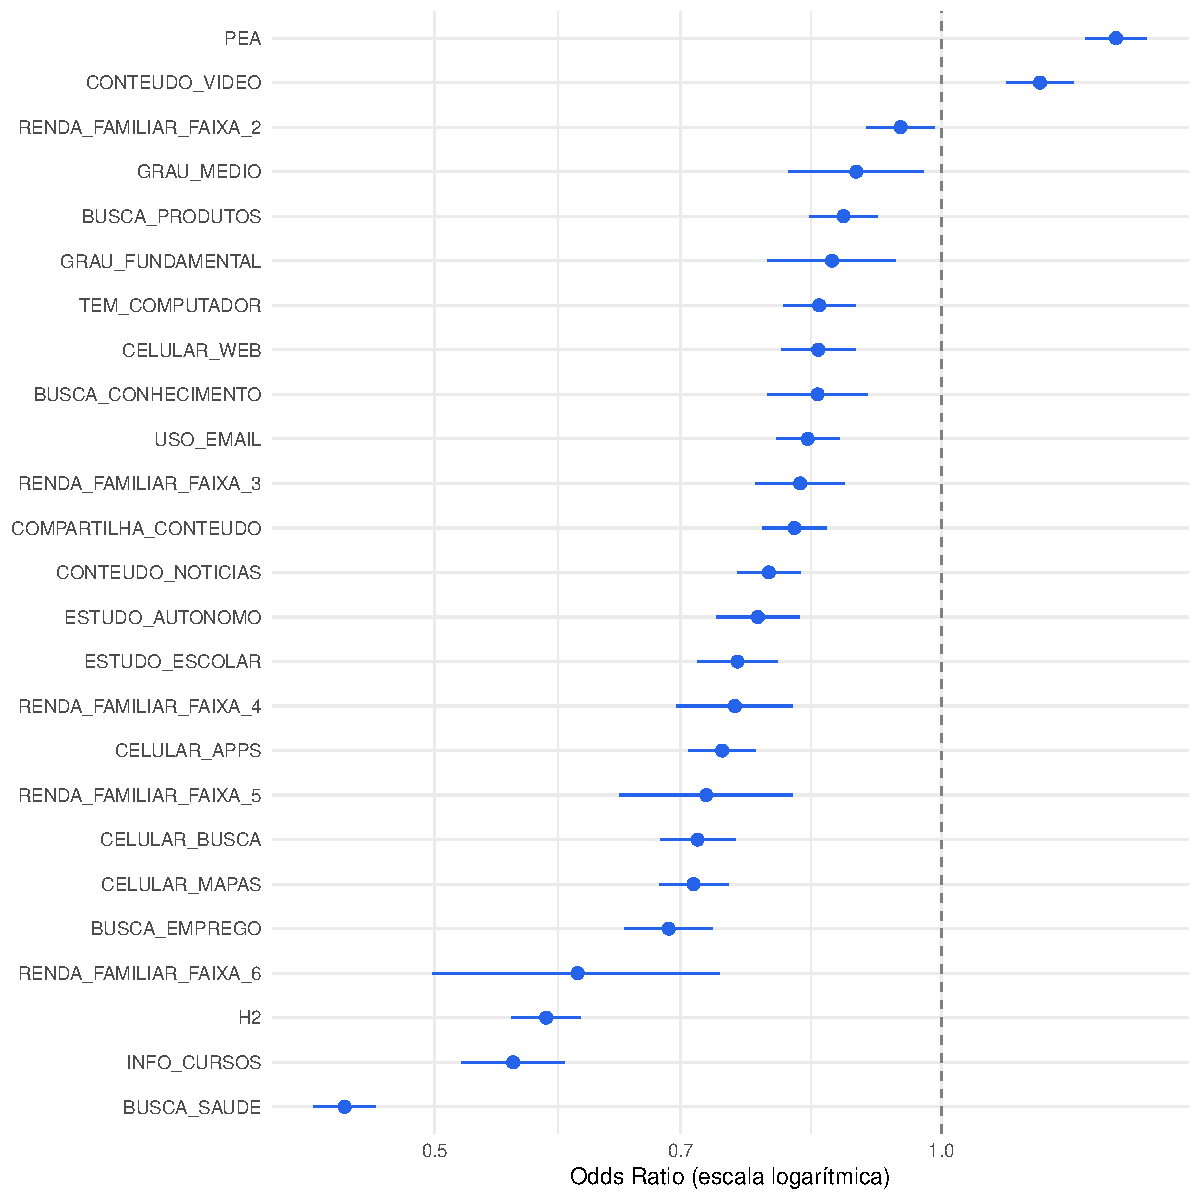
\includegraphics[keepaspectratio]{artigo_files/figure-pdf/fig-or-1.pdf}}

}

\end{figure}%

A Figura~\ref{fig-importancia} apresenta a importância relativa das
variáveis no Random Forest Expandido (medida de impureza Gini,
normalizada). A ordenação confirma o padrão observado nos \emph{odds
ratios} da regressão logística: variáveis de prática digital ocupam as
primeiras posições, com \texttt{BUSCA\_SAUDE} no topo, seguida por idade
e variáveis de uso intenso de celular e de informação. A coerência entre
os dois métodos sobre o mesmo conjunto de variáveis reforça que o sinal
preditivo está nas variáveis, não no modelo.

\begin{figure}

\caption{\label{fig-importancia}Importância das variáveis no Random
Forest Expandido (impureza Gini, normalizada)}

\centering{

\pandocbounded{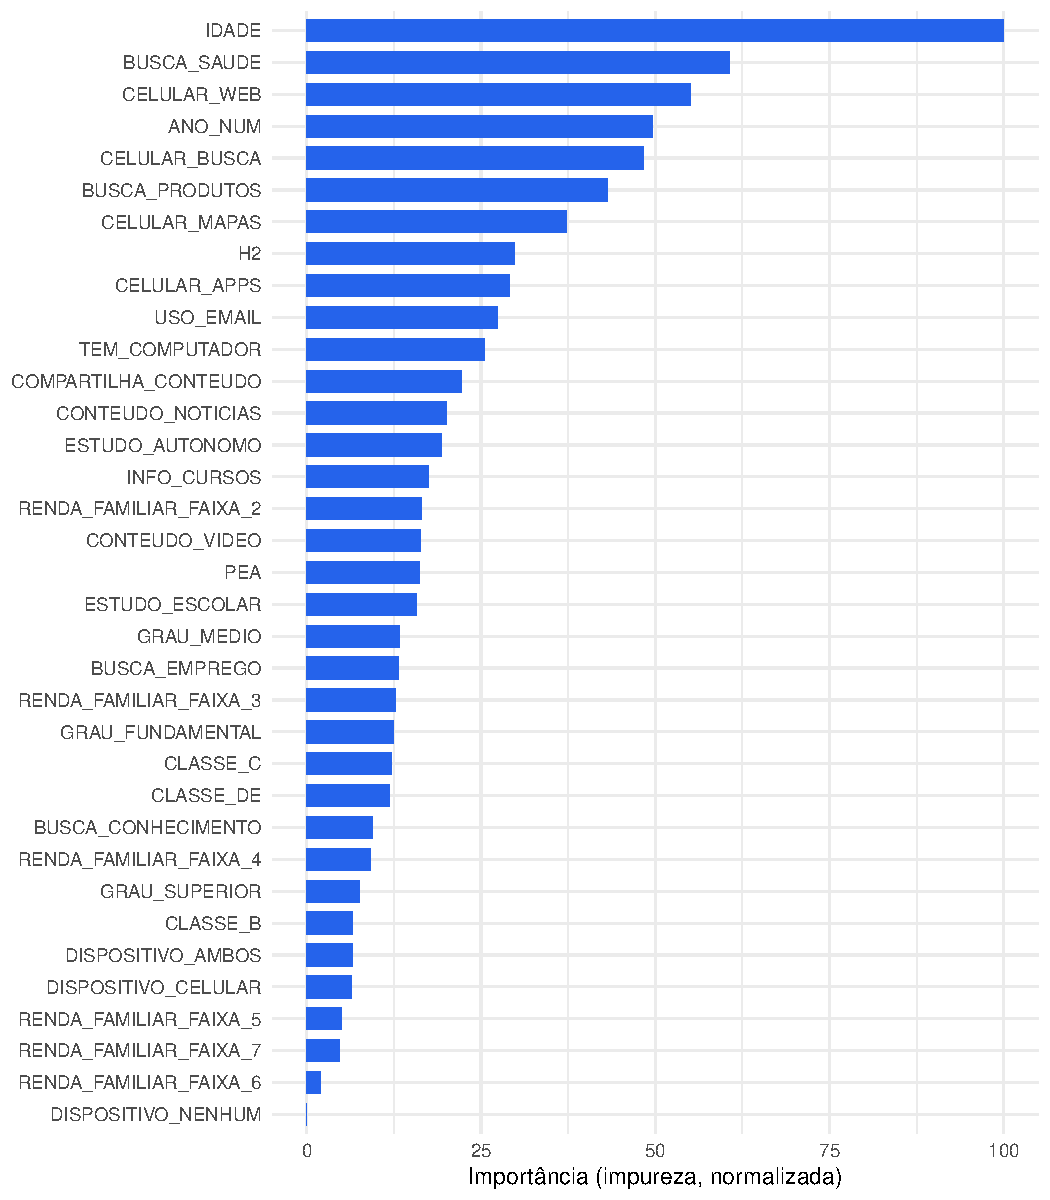
\includegraphics[keepaspectratio]{artigo_files/figure-pdf/fig-importancia-1.pdf}}

}

\end{figure}%

\subsubsection{Generalização temporal: holdout em
2025}\label{generalizauxe7uxe3o-temporal-holdout-em-2025}

Para verificar a estabilidade dos efeitos estimados, os modelos foram
retreinados em 2021-2024 e testados na edição de 2025 cega ao processo
de estimação. A Tabela~\ref{tbl-holdout} apresenta os resultados.

\begin{table}

{\caption{{Desempenho dos modelos no holdout temporal (treino 2021-2024;
teste na edição 2025)}{\label{tbl-holdout}}}
\vspace{-20pt}}

\global\setlength{\Oldarrayrulewidth}{\arrayrulewidth}

\global\setlength{\Oldtabcolsep}{\tabcolsep}

\setlength{\tabcolsep}{2pt}

\renewcommand*{\arraystretch}{1.5}



\providecommand{\ascline}[3]{\noalign{\global\arrayrulewidth #1}\arrayrulecolor[HTML]{#2}\cline{#3}}

\begin{longtable*}[c]{|p{1.18in}|p{0.57in}|p{0.59in}|p{0.74in}|p{0.57in}}



\ascline{1.5pt}{666666}{1-5}

\multicolumn{1}{>{\raggedright}m{\dimexpr 1.18in+0\tabcolsep}}{\textcolor[HTML]{000000}{\fontsize{9}{9}\selectfont{\global\setmainfont{DejaVu Sans}{Modelo}}}} & \multicolumn{1}{>{\raggedleft}m{\dimexpr 0.57in+0\tabcolsep}}{\textcolor[HTML]{000000}{\fontsize{9}{9}\selectfont{\global\setmainfont{DejaVu Sans}{AUC}}}} & \multicolumn{1}{>{\raggedleft}m{\dimexpr 0.59in+0\tabcolsep}}{\textcolor[HTML]{000000}{\fontsize{9}{9}\selectfont{\global\setmainfont{DejaVu Sans}{Recall}}}} & \multicolumn{1}{>{\raggedleft}m{\dimexpr 0.74in+0\tabcolsep}}{\textcolor[HTML]{000000}{\fontsize{9}{9}\selectfont{\global\setmainfont{DejaVu Sans}{Precisão}}}} & \multicolumn{1}{>{\raggedleft}m{\dimexpr 0.57in+0\tabcolsep}}{\textcolor[HTML]{000000}{\fontsize{9}{9}\selectfont{\global\setmainfont{DejaVu Sans}{F1}}}} \\

\ascline{1.5pt}{666666}{1-5}\endfirsthead 

\ascline{1.5pt}{666666}{1-5}

\multicolumn{1}{>{\raggedright}m{\dimexpr 1.18in+0\tabcolsep}}{\textcolor[HTML]{000000}{\fontsize{9}{9}\selectfont{\global\setmainfont{DejaVu Sans}{Modelo}}}} & \multicolumn{1}{>{\raggedleft}m{\dimexpr 0.57in+0\tabcolsep}}{\textcolor[HTML]{000000}{\fontsize{9}{9}\selectfont{\global\setmainfont{DejaVu Sans}{AUC}}}} & \multicolumn{1}{>{\raggedleft}m{\dimexpr 0.59in+0\tabcolsep}}{\textcolor[HTML]{000000}{\fontsize{9}{9}\selectfont{\global\setmainfont{DejaVu Sans}{Recall}}}} & \multicolumn{1}{>{\raggedleft}m{\dimexpr 0.74in+0\tabcolsep}}{\textcolor[HTML]{000000}{\fontsize{9}{9}\selectfont{\global\setmainfont{DejaVu Sans}{Precisão}}}} & \multicolumn{1}{>{\raggedleft}m{\dimexpr 0.57in+0\tabcolsep}}{\textcolor[HTML]{000000}{\fontsize{9}{9}\selectfont{\global\setmainfont{DejaVu Sans}{F1}}}} \\

\ascline{1.5pt}{666666}{1-5}\endhead



\multicolumn{1}{>{\raggedright}m{\dimexpr 1.18in+0\tabcolsep}}{\textcolor[HTML]{000000}{\fontsize{9}{9}\selectfont{\global\setmainfont{DejaVu Sans}{GLM\ Original}}}} & \multicolumn{1}{>{\raggedleft}m{\dimexpr 0.57in+0\tabcolsep}}{\textcolor[HTML]{000000}{\fontsize{9}{9}\selectfont{\global\setmainfont{DejaVu Sans}{0.772}}}} & \multicolumn{1}{>{\raggedleft}m{\dimexpr 0.59in+0\tabcolsep}}{\textcolor[HTML]{000000}{\fontsize{9}{9}\selectfont{\global\setmainfont{DejaVu Sans}{0.649}}}} & \multicolumn{1}{>{\raggedleft}m{\dimexpr 0.74in+0\tabcolsep}}{\textcolor[HTML]{000000}{\fontsize{9}{9}\selectfont{\global\setmainfont{DejaVu Sans}{0.841}}}} & \multicolumn{1}{>{\raggedleft}m{\dimexpr 0.57in+0\tabcolsep}}{\textcolor[HTML]{000000}{\fontsize{9}{9}\selectfont{\global\setmainfont{DejaVu Sans}{0.732}}}} \\





\multicolumn{1}{>{\raggedright}m{\dimexpr 1.18in+0\tabcolsep}}{\textcolor[HTML]{000000}{\fontsize{9}{9}\selectfont{\global\setmainfont{DejaVu Sans}{GLM\ Expandido}}}} & \multicolumn{1}{>{\raggedleft}m{\dimexpr 0.57in+0\tabcolsep}}{\textcolor[HTML]{000000}{\fontsize{9}{9}\selectfont{\global\setmainfont{DejaVu Sans}{0.835}}}} & \multicolumn{1}{>{\raggedleft}m{\dimexpr 0.59in+0\tabcolsep}}{\textcolor[HTML]{000000}{\fontsize{9}{9}\selectfont{\global\setmainfont{DejaVu Sans}{0.680}}}} & \multicolumn{1}{>{\raggedleft}m{\dimexpr 0.74in+0\tabcolsep}}{\textcolor[HTML]{000000}{\fontsize{9}{9}\selectfont{\global\setmainfont{DejaVu Sans}{0.882}}}} & \multicolumn{1}{>{\raggedleft}m{\dimexpr 0.57in+0\tabcolsep}}{\textcolor[HTML]{000000}{\fontsize{9}{9}\selectfont{\global\setmainfont{DejaVu Sans}{0.768}}}} \\





\multicolumn{1}{>{\raggedright}m{\dimexpr 1.18in+0\tabcolsep}}{\textcolor[HTML]{000000}{\fontsize{9}{9}\selectfont{\global\setmainfont{DejaVu Sans}{RF\ Original}}}} & \multicolumn{1}{>{\raggedleft}m{\dimexpr 0.57in+0\tabcolsep}}{\textcolor[HTML]{000000}{\fontsize{9}{9}\selectfont{\global\setmainfont{DejaVu Sans}{0.767}}}} & \multicolumn{1}{>{\raggedleft}m{\dimexpr 0.59in+0\tabcolsep}}{\textcolor[HTML]{000000}{\fontsize{9}{9}\selectfont{\global\setmainfont{DejaVu Sans}{0.653}}}} & \multicolumn{1}{>{\raggedleft}m{\dimexpr 0.74in+0\tabcolsep}}{\textcolor[HTML]{000000}{\fontsize{9}{9}\selectfont{\global\setmainfont{DejaVu Sans}{0.833}}}} & \multicolumn{1}{>{\raggedleft}m{\dimexpr 0.57in+0\tabcolsep}}{\textcolor[HTML]{000000}{\fontsize{9}{9}\selectfont{\global\setmainfont{DejaVu Sans}{0.732}}}} \\





\multicolumn{1}{>{\raggedright}m{\dimexpr 1.18in+0\tabcolsep}}{\textcolor[HTML]{000000}{\fontsize{9}{9}\selectfont{\global\setmainfont{DejaVu Sans}{RF\ Expandido}}}} & \multicolumn{1}{>{\raggedleft}m{\dimexpr 0.57in+0\tabcolsep}}{\textcolor[HTML]{000000}{\fontsize{9}{9}\selectfont{\global\setmainfont{DejaVu Sans}{0.829}}}} & \multicolumn{1}{>{\raggedleft}m{\dimexpr 0.59in+0\tabcolsep}}{\textcolor[HTML]{000000}{\fontsize{9}{9}\selectfont{\global\setmainfont{DejaVu Sans}{0.726}}}} & \multicolumn{1}{>{\raggedleft}m{\dimexpr 0.74in+0\tabcolsep}}{\textcolor[HTML]{000000}{\fontsize{9}{9}\selectfont{\global\setmainfont{DejaVu Sans}{0.863}}}} & \multicolumn{1}{>{\raggedleft}m{\dimexpr 0.57in+0\tabcolsep}}{\textcolor[HTML]{000000}{\fontsize{9}{9}\selectfont{\global\setmainfont{DejaVu Sans}{0.789}}}} \\

\ascline{1.5pt}{666666}{1-5}



\end{longtable*}



\arrayrulecolor[HTML]{000000}

\global\setlength{\arrayrulewidth}{\Oldarrayrulewidth}

\global\setlength{\tabcolsep}{\Oldtabcolsep}

\renewcommand*{\arraystretch}{1}

\end{table}

O AUC do GLM Expandido em 2025 cego é de aproximadamente 0,835,
ligeiramente superior ao AUC obtido em validação cruzada \emph{pooled}
(0,831). A diferença é de magnitude desprezível, sugerindo que os
efeitos estimados não dependem de particularidades dos anos de treino e
generalizam para o ano subsequente.

\subsubsection{Sensibilidade: habilidades digitais e estimação
ponderada}\label{sensibilidade-habilidades-digitais-e-estimauxe7uxe3o-ponderada}

Duas análises complementam o achado principal.

A primeira inclui as 12 variáveis de \textbf{habilidades digitais
autorelatadas} (I1A\_\emph{) sobre os anos de 2022-2025 (n ≈ 56 mil), em
que as variáveis estão disponíveis. O AUC do GLM expandido sem I1A\_}
sobre essa subamostra é de aproximadamente 0,831; com I1A\_\emph{, sobe
para 0,839 (ΔAUC = +0,008). O Random Forest com I1A\_} atinge AUC de
0,842 (ΔAUC = +0,010 sobre o RF expandido sem I1A\_*). O ganho marginal
pequeno indica que as 16 práticas digitais incluídas no modelo expandido
já absorvem a maior parte do espaço de habilidades, leitura coerente com
a noção teórica de \textbf{familiaridade digital}
(\citeproc{ref-ebbers2016impactof}{Ebbers; Jansen; Deursen, 2016};
\citeproc{ref-lutz2019digitali}{Lutz, 2019}), em que prática frequente e
variada converge funcionalmente com habilidades autorelatadas.

A segunda análise estima o GLM Expandido com \textbf{pesos amostrais} da
TIC Domicílios via \emph{svyglm}, comparando os coeficientes ponderados
com os não ponderados. Os coeficientes das 16 variáveis de prática
digital mantêm sinal e significância em ambas as estimações; a diferença
mediana em log-\emph{odds} entre as duas estimativas é da ordem de 0,03
em valor absoluto. Algumas variáveis sociodemográficas (CLASSE\_CB e
níveis de C5\_DISPOSITIVOS) perdem significância na estimação ponderada,
mas o efeito principal das variáveis de prática digital permanece
robusto. O resultado valida o uso da estimação não ponderada como modelo
principal sem prejuízo substancial.

\subsection{Discussão}\label{discussuxe3o}

\subsubsection{A prática digital cotidiana complementa o perfil
sociodemográfico}\label{a-pruxe1tica-digital-cotidiana-complementa-o-perfil-sociodemogruxe1fico}

O resultado principal, isto é, o ganho de AUC de aproximadamente seis
pontos com a inclusão das 16 variáveis de prática digital cotidiana,
oferece evidência direta de que a prática digital complementa, em vez de
substituir, o perfil sociodemográfico na explicação da adoção de e-gov
no Brasil. As variáveis sociodemográficas tradicionais permanecem com
efeitos estatisticamente significativos no modelo expandido, mas seu
poder explicativo é incrementado pela inclusão de práticas específicas.
O resultado é coerente com a previsão teórica de Büchi; Just; Latzer
(\citeproc{ref-bchi2016modeling}{2016}) de que sociodemográficas
explicam até cerca de metade da variância no uso da internet em
populações com acesso amplo, deixando espaço para preditores ligados a
habilidades e tipos de uso. Em terreno brasileiro, esse ``espaço de
variância'' começa a ser preenchido empiricamente com a evidência aqui
reportada.

A coerência entre os \emph{odds ratios} da regressão logística e a
importância relativa das variáveis no Random Forest, ambos identificando
práticas digitais como preditores principais, sugere que o efeito é
estrutural (i.e., atribuível ao conjunto de variáveis) e não dependente
da classe de modelo escolhida. A Figura~\ref{fig-or} e a
Figura~\ref{fig-importancia}, comparadas, mostram convergência
substantiva sobre quais práticas mais pesam na adoção: busca de
informação especializada (saúde, cursos), uso ativo do celular para
mapas e \emph{apps}, e atividades educacionais.

\subsubsection{\texorpdfstring{Diálogo cumulativo com Vargas et al.
(\citeproc{ref-vargas2021}{2021}) e Dodel
(\citeproc{ref-dodel2023whydevic}{2023})}{Diálogo cumulativo com Vargas et al. (2021) e Dodel (2023)}}\label{diuxe1logo-cumulativo-com-vargas2021-e-dodel2023whydevic}

Esta análise estende o trabalho de Vargas et al.
(\citeproc{ref-vargas2021}{2021}) em duas direções complementares. Na
primeira, atende a uma sugestão explícita dos próprios autores em suas
considerações finais (testar características de uso específicas além da
agregação adotada para a variável dependente), incorporando 16 dimensões
de prática digital cotidiana. Na segunda, amplia a janela temporal de
uma única edição (2019) para o pooled 2021-2025, captando o contexto
pós-pandemia, em que práticas digitais ganharam centralidade frente a
serviços tradicionais.

Dodel (\citeproc{ref-dodel2023whydevic}{2023}) abriu, no Brasil, a
frente empírica de ``prática digital media o efeito do perfil
socioeconômico'' ao examinar o dispositivo de acesso (computador versus
apenas celular) com microdados da TIC Domicílios 2019 e o framework
DiSTO. Nossa análise complementa essa contribuição cumulativa em três
aspectos: (i) examina uma variedade ampla de práticas digitais
cotidianas, não restrita ao dispositivo; (ii) cobre janela longitudinal
pós-pandemia; (iii) avalia estabilidade temporal por holdout em ano
cego. A leitura conjunta dos achados aponta para um quadro coerente: o
uso da internet pelo cidadão, seja medido pelo dispositivo, seja pela
variedade de atividades específicas, opera como camada estruturante da
adoção de e-gov no Brasil, complementando os efeitos do perfil
sociodemográfico mapeados pela literatura anterior.

\subsubsection{Familiaridade digital como
construto}\label{familiaridade-digital-como-construto}

A análise de sensibilidade com habilidades digitais autorelatadas
(I1A\_*) traz uma evidência conceitual relevante. O ganho marginal de
AUC ao incluir habilidades é da ordem de 0,008 a 0,010, modesto frente
ao ganho de seis pontos das 16 práticas. Uma leitura coerente com a
literatura é a de \textbf{familiaridade digital} como construto
convergente: prática frequente e variada da internet aproxima-se
funcionalmente do conceito de habilidade autorrelatada, isto é, quem
realiza atividades digitais cotidianas reporta-se mais hábil, e o
conjunto de práticas observadas captura grande parte do que a
autorrelato de habilidades adicionaria como informação. Esse é o sentido
em que Ebbers; Jansen; Deursen (\citeproc{ref-ebbers2016impactof}{2016})
falam do deslocamento ``de \emph{channel choice} para \emph{channel
usage}'': é o uso, e não a posse de habilidade declarada, que diferencia
adoção quando há acesso.

\subsubsection{Pandemia, Auxílio Emergencial e implicações para o
Brasil}\label{pandemia-auxuxedlio-emergencial-e-implicauxe7uxf5es-para-o-brasil}

A janela 2021-2025 capta o contexto pós-pandêmico, em que o Auxílio
Emergencial e a transformação digital de outros serviços públicos
forçaram o engajamento de populações historicamente menos familiarizadas
com canais digitais. Cardoso (\citeproc{ref-cardoso2020aimpleme}{2020})
caracteriza esse momento como exemplo de ``\emph{system-level
bureaucracy}'', em que decisões pré-programadas via algoritmos passaram
a operar serviços públicos em escala. A leitura empírica que esta
análise oferece complementa o relato qualitativo: o conjunto de práticas
digitais mantém papel central na adoção de e-gov mesmo após o salto na
oferta digitalizada, e os efeitos estimados são estáveis temporalmente.
A pandemia, em vez de reduzir a importância da prática digital cotidiana
(pela hipótese de familiarização forçada), parece ter reforçado seu
papel preditivo, em consonância com o achado de Deursen
(\citeproc{ref-vandeursen2020digitali}{2020}) em contexto holandês.

\subsubsection{Implicação
metodológica}\label{implicauxe7uxe3o-metodoluxf3gica}

Um achado secundário, mas relevante para a prática de pesquisa empírica
em e-gov, é a equivalência de desempenho entre regressão logística,
Random Forest e árvore de decisão sobre o mesmo conjunto de variáveis.
As três técnicas, sobre os preditores expandidos, atingem AUC
praticamente idêntico (cerca de 0,83). A leitura correta não é ``o
método não importa em geral'', mas sim que, para este desfecho com este
conjunto de preditores, o sinal preditivo é majoritariamente linear no
espaço ampliado. A escolha entre métodos pode então ser orientada por
critérios de interpretabilidade (favorecendo a regressão logística, que
oferece \emph{odds ratios} diretamente comparáveis com a literatura
tradicional) sem prejuízo de poder preditivo. Essa observação é coerente
com o que Browne; Matteson; McBride
(\citeproc{ref-browne2021multivar}{2021}) e Sohnesen; Stender
(\citeproc{ref-mcbride2017israndom}{2017}) encontraram em domínios
distintos (pobreza, malnutrição) e dialoga com o debate sobre quando
\emph{machine learning} mais flexível agrega valor frente a modelos
lineares tradicionais.

\subsubsection{Limitações}\label{limitauxe7uxf5es}

Quatro limitações merecem registro. Primeira, a estimação principal não
incorpora pesos amostrais; a análise de sensibilidade via \emph{svyglm}
indica robustez dos efeitos das variáveis de prática digital, mas a
generalização para a população brasileira como um todo deve considerar a
estrutura amostral complexa da TIC Domicílios. Segunda, o desfecho
G1\_AGREG é uma agregação binária de 29 questões; uma análise de
sensibilidade desagregada por tipo de serviço (declaração de imposto,
agendamento médico, matrícula escolar) seria informativa, mas excede o
escopo deste artigo. Terceira, a edição de 2025 incluiu uma nova questão
sobre serviços de Justiça (G1\_H), o que pode inflacionar levemente a
proporção de uso comparativamente aos anos anteriores. Quarta, a relação
entre perfil sociodemográfico e prática digital (adição, mediação,
moderação) não foi formalmente decomposta por análise de mediação. A
literatura indica que mediação é provável
(\citeproc{ref-dodel2023whydevic}{Dodel, 2023}), e o teste rigoroso
desse mecanismo permanece como direção promissora para pesquisa futura.

\subsection{Conclusão e
implicações}\label{conclusuxe3o-e-implicauxe7uxf5es}

Este estudo investigou em que medida a prática digital cotidiana
complementa o perfil sociodemográfico na explicação da adoção de governo
eletrônico no Brasil pós-pandemia. Os achados apontam para uma resposta
clara: a prática digital adiciona substancialmente ao poder explicativo
do perfil sociodemográfico, com ganho de aproximadamente seis pontos de
AUC sobre o modelo de Vargas et al. (\citeproc{ref-vargas2021}{2021}) e
estabilidade temporal validada por holdout em 2025.

Em termos teóricos, a contribuição é a de oferecer evidência empírica
brasileira para o deslocamento conceitual, previsto pela literatura
internacional de divisão digital, do plano do acesso ao plano do uso. As
16 dimensões de prática digital cotidiana operam como construto
coerente, coerente com a noção de familiaridade digital, e ocupam parte
expressiva do ``espaço de variância'' deixado pelas variáveis
sociodemográficas tradicionais.

Em termos práticos, o achado tem implicações para políticas de e-gov:
ampliar a adoção depende não apenas de políticas redistributivas que
alterem o perfil sociodemográfico (renda, escolaridade), mas também de
iniciativas que estimulem práticas digitais cotidianas, como letramento
digital aplicado, ofertas de informação online em domínios como saúde e
educação e integração de serviços com aplicativos móveis comuns. A
pandemia mostrou que a aceleração da oferta digital, isoladamente, não
basta: é a familiaridade do cidadão com práticas digitais cotidianas que
viabiliza a apropriação dos serviços.

Direções para pesquisa futura incluem o teste formal de mediação entre
perfil sociodemográfico, prática digital e adoção de e-gov; a análise
desagregada por tipo de serviço público; e a comparação com países
latino-americanos com microdados similares, em diálogo com a agenda de
Gray; Gainous; Wagner (\citeproc{ref-hilbert2016genderan}{2016}) e
Reisdorf (\citeproc{ref-reisdorf2021whenbein}{2021}).

\subsection{Apêndice}\label{apuxeandice}

\subsubsection{Código central de treinamento dos
modelos}\label{cuxf3digo-central-de-treinamento-dos-modelos}

O treinamento dos modelos foi realizado em três scripts standalone
(\texttt{scripts/fit\_ml.R}, \texttt{scripts/fit\_i1a.R} e
\texttt{scripts/fit\_svyglm.R}), com saída em arquivos RDS lidos por
este artigo. Reproduzem-se a seguir os trechos centrais para fins de
transparência metodológica; o código completo está disponível no
notebook técnico que acompanha o artigo.

\begin{codelisting}

\caption{\texttt{scripts/fit\_ml.R (excerto)}}

\begin{Shaded}
\begin{Highlighting}[]
\CommentTok{\# Variáveis do artigo de referência (Vargas et al., 2021)}
\NormalTok{vars\_art }\OtherTok{\textless{}{-}} \FunctionTok{c}\NormalTok{(}\StringTok{"IDADE"}\NormalTok{, }\StringTok{"PEA"}\NormalTok{, }\StringTok{"H2"}\NormalTok{, }\StringTok{"RENDA\_FAMILIAR"}\NormalTok{, }\StringTok{"CLASSE\_CB"}\NormalTok{,}
              \StringTok{"GRAU\_INSTRUCAO"}\NormalTok{, }\StringTok{"C5\_DISPOSITIVOS"}\NormalTok{)}
\NormalTok{vars\_categoricas }\OtherTok{\textless{}{-}} \FunctionTok{c}\NormalTok{(}\StringTok{"RENDA\_FAMILIAR"}\NormalTok{, }\StringTok{"CLASSE\_CB"}\NormalTok{, }\StringTok{"GRAU\_INSTRUCAO"}\NormalTok{,}
                      \StringTok{"C5\_DISPOSITIVOS"}\NormalTok{)}

\CommentTok{\# 16 variáveis de prática digital cotidiana (selecionadas por screening)}
\CommentTok{\# Códigos TIC originais renomeados em scripts/var\_labels.R para nomes}
\CommentTok{\# interpretáveis (BUSCA\_SAUDE, CELULAR\_MAPAS, ESTUDO\_AUTONOMO, ...)}
\FunctionTok{source}\NormalTok{(}\StringTok{"scripts/var\_labels.R"}\NormalTok{)}

\CommentTok{\# Folds fixos para comparação pareada entre modelos}
\NormalTok{folds }\OtherTok{\textless{}{-}}\NormalTok{ caret}\SpecialCharTok{::}\FunctionTok{createFolds}\NormalTok{(df}\SpecialCharTok{$}\NormalTok{egov, }\AttributeTok{k =} \DecValTok{5}\NormalTok{, }\AttributeTok{returnTrain =} \ConstantTok{TRUE}\NormalTok{)}
\NormalTok{ctrl  }\OtherTok{\textless{}{-}}\NormalTok{ caret}\SpecialCharTok{::}\FunctionTok{trainControl}\NormalTok{(}\AttributeTok{method =} \StringTok{"cv"}\NormalTok{, }\AttributeTok{number =} \DecValTok{5}\NormalTok{, }\AttributeTok{index =}\NormalTok{ folds,}
                             \AttributeTok{classProbs =} \ConstantTok{TRUE}\NormalTok{,}
                             \AttributeTok{summaryFunction =}\NormalTok{ caret}\SpecialCharTok{::}\NormalTok{twoClassSummary,}
                             \AttributeTok{savePredictions =} \StringTok{"final"}\NormalTok{)}

\CommentTok{\# Cinco modelos sobre o mesmo N e mesmas folds}
\NormalTok{glm\_orig }\OtherTok{\textless{}{-}}\NormalTok{ caret}\SpecialCharTok{::}\FunctionTok{train}\NormalTok{(egov }\SpecialCharTok{\textasciitilde{}}\NormalTok{ ., }\AttributeTok{data =}\NormalTok{ df\_orig, }\AttributeTok{method =} \StringTok{"glm"}\NormalTok{,}
                         \AttributeTok{family =} \StringTok{"binomial"}\NormalTok{, }\AttributeTok{trControl =}\NormalTok{ ctrl, }\AttributeTok{metric =} \StringTok{"ROC"}\NormalTok{)}
\NormalTok{glm\_exp  }\OtherTok{\textless{}{-}}\NormalTok{ caret}\SpecialCharTok{::}\FunctionTok{train}\NormalTok{(egov }\SpecialCharTok{\textasciitilde{}}\NormalTok{ ., }\AttributeTok{data =}\NormalTok{ df\_exp,  }\AttributeTok{method =} \StringTok{"glm"}\NormalTok{,}
                         \AttributeTok{family =} \StringTok{"binomial"}\NormalTok{, }\AttributeTok{trControl =}\NormalTok{ ctrl, }\AttributeTok{metric =} \StringTok{"ROC"}\NormalTok{)}
\NormalTok{tree     }\OtherTok{\textless{}{-}}\NormalTok{ caret}\SpecialCharTok{::}\FunctionTok{train}\NormalTok{(egov }\SpecialCharTok{\textasciitilde{}}\NormalTok{ ., }\AttributeTok{data =}\NormalTok{ df\_orig, }\AttributeTok{method =} \StringTok{"rpart"}\NormalTok{,}
                         \AttributeTok{trControl =}\NormalTok{ ctrl, }\AttributeTok{metric =} \StringTok{"ROC"}\NormalTok{)}
\NormalTok{rf\_orig  }\OtherTok{\textless{}{-}}\NormalTok{ caret}\SpecialCharTok{::}\FunctionTok{train}\NormalTok{(egov }\SpecialCharTok{\textasciitilde{}}\NormalTok{ ., }\AttributeTok{data =}\NormalTok{ df\_orig, }\AttributeTok{method =} \StringTok{"ranger"}\NormalTok{,}
                         \AttributeTok{trControl =}\NormalTok{ ctrl, }\AttributeTok{metric =} \StringTok{"ROC"}\NormalTok{,}
                         \AttributeTok{num.trees =} \DecValTok{300}\NormalTok{, }\AttributeTok{num.threads =} \DecValTok{1}\NormalTok{)}
\NormalTok{rf\_exp   }\OtherTok{\textless{}{-}}\NormalTok{ caret}\SpecialCharTok{::}\FunctionTok{train}\NormalTok{(egov }\SpecialCharTok{\textasciitilde{}}\NormalTok{ ., }\AttributeTok{data =}\NormalTok{ df\_exp,  }\AttributeTok{method =} \StringTok{"ranger"}\NormalTok{,}
                         \AttributeTok{trControl =}\NormalTok{ ctrl, }\AttributeTok{metric =} \StringTok{"ROC"}\NormalTok{,}
                         \AttributeTok{num.trees =} \DecValTok{300}\NormalTok{, }\AttributeTok{num.threads =} \DecValTok{1}\NormalTok{)}
\end{Highlighting}
\end{Shaded}

\end{codelisting}

\begin{codelisting}

\caption{\texttt{scripts/fit\_i1a.R (excerto)}}

\begin{Shaded}
\begin{Highlighting}[]
\CommentTok{\# Habilidades digitais autorelatadas (12 itens, disponíveis a partir de 2022).}
\CommentTok{\# "Não sei / Não respondeu" (códigos 97/98/99) é tratado como ausência da}
\CommentTok{\# habilidade (0), evitando perda massiva de N por drop\_na.}
\NormalTok{vars\_i1a }\OtherTok{\textless{}{-}} \FunctionTok{c}\NormalTok{(}\StringTok{"I1A\_A"}\NormalTok{,}\StringTok{"I1A\_B"}\NormalTok{,}\StringTok{"I1A\_C"}\NormalTok{,}\StringTok{"I1A\_D"}\NormalTok{,}\StringTok{"I1A\_E"}\NormalTok{,}\StringTok{"I1A\_F"}\NormalTok{,}
              \StringTok{"I1A\_G"}\NormalTok{,}\StringTok{"I1A\_H"}\NormalTok{,}\StringTok{"I1A\_I"}\NormalTok{,}\StringTok{"I1A\_J"}\NormalTok{,}\StringTok{"I1A\_K"}\NormalTok{,}\StringTok{"I1A\_L"}\NormalTok{)}

\NormalTok{recode\_hab }\OtherTok{\textless{}{-}} \ControlFlowTok{function}\NormalTok{(x) \{}
\NormalTok{  x }\OtherTok{\textless{}{-}} \FunctionTok{as.numeric}\NormalTok{(x)}
\NormalTok{  x[x }\SpecialCharTok{\%in\%} \FunctionTok{c}\NormalTok{(}\DecValTok{97}\NormalTok{, }\DecValTok{98}\NormalTok{, }\DecValTok{99}\NormalTok{)] }\OtherTok{\textless{}{-}} \DecValTok{0}
\NormalTok{  x}
\NormalTok{\}}

\NormalTok{pool }\OtherTok{\textless{}{-}}\NormalTok{ pool }\SpecialCharTok{|\textgreater{}}
  \FunctionTok{mutate}\NormalTok{(}\FunctionTok{across}\NormalTok{(}\FunctionTok{all\_of}\NormalTok{(vars\_i1a), recode\_hab))}
\end{Highlighting}
\end{Shaded}

\end{codelisting}

\subsection{Referências}\label{referuxeancias}

\protect\phantomsection\label{refs}
\begin{CSLReferences}{0}{1}
\bibitem[\citeproctext]{ref-araujo2018servicos}
ARAUJO. \href{https://doi.org/10.1590/0034-7612171925}{Servicos de
governo eletronico no Brasil: uma analise a partir das medidas de acesso
e competencias de uso da internet}. 2018.

\bibitem[\citeproctext]{ref-araujoreinha2015contextu}
ARAUJOREINHARD. \href{https://doi.org/10.5700/rege579}{Contextual
factors that influence the adoption of e-government in Brazil}. 2015.

\bibitem[\citeproctext]{ref-belanger2008trustand}
BELANGER. \href{https://doi.org/10.1016/j.jsis.2007.12.002}{Trust and
risk in e-government adoption}. 2008.

\bibitem[\citeproctext]{ref-browne2021multivar}
BROWNE, Chris; MATTESON, David S.; MCBRIDE, Linden.
\href{https://doi.org/10.1371/journal.pone.0255519}{Multivariate random
forest prediction of poverty and malnutrition prevalence}. \textbf{Plos
One}, 2021.

\bibitem[\citeproctext]{ref-bchi2016modeling}
BÜCHI, Moritz; JUST, Natascha; LATZER, Michael.
\href{https://doi.org/10.1177/1461444815604154}{Modeling the
second-level digital divide: A five-country study of social differences
in Internet use}. \textbf{New Media \& Society}, 2016.

\bibitem[\citeproctext]{ref-cardoso2020aimpleme}
CARDOSO. \href{https://doi.org/10.1590/0034-761220200267}{A
implementacao do Auxilio Emergencial como medida excepcional de protecao
social}. 2020.

\bibitem[\citeproctext]{ref-castellacci2018internet}
CASTELLACCI, Fulvio; TVEITO, Vegard.
\href{https://doi.org/10.1016/j.respol.2017.11.007}{Internet use and
well-being: A survey and a theoretical framework}. \textbf{Research
Policy}, 2018.

\bibitem[\citeproctext]{ref-cetic2025}
CETIC.BR. \textbf{{TIC} {D}omicílios 2015-2025: microdados}. Centro
Regional de Estudos para o Desenvolvimento da Sociedade da Informação,
2025. Disponível em:
\textless{}\url{https://cetic.br/pt/pesquisa/domicilios/microdados/}\textgreater{}

\bibitem[\citeproctext]{ref-R-doParallel}
CORPORATION, Microsoft; WESTON, Steve.
\textbf{\href{https://github.com/RevolutionAnalytics/doparallel}{doParallel:
Foreach Parallel Adaptor for the parallel Package}}. \emph{{[}S.l.:
S.n.{]}}.

\bibitem[\citeproctext]{ref-davis1989perceive}
DAVIS. \href{https://doi.org/10.2307/249008}{Perceived usefulness,
perceived ease of use, and user acceptance of information technology}.
1989.

\bibitem[\citeproctext]{ref-vandeursen2020digitali}
DEURSEN, Alexander Johannes Aloysius Maria van.
\href{https://doi.org/10.2196/20073}{Digital Inequality During a
Pandemic: Quantitative Study of Differences in COVID-19--Related
Internet Uses and Outcomes Among the General Population}.
\textbf{Journal of Medical Internet Research}, 2020.

\bibitem[\citeproctext]{ref-dodel2023whydevic}
DODEL, Matías. \href{https://doi.org/10.1177/08944393231176595}{Why
Device-Related Digital Inequalities Matter for E-Government Engagement?}
\textbf{Social Science Computer Review}, 2023.

\bibitem[\citeproctext]{ref-ebbers2016impactof}
EBBERS, Wolfgang E.; JANSEN, Marloes; DEURSEN, Alexander Johannes
Aloysius Maria van.
\href{https://doi.org/10.1016/j.giq.2016.08.007}{Impact of the digital
divide on e-government: Expanding from channel choice to channel usage}.
\textbf{Government Information Quarterly}, 2016.

\bibitem[\citeproctext]{ref-R-survey}
GAO, Peter; SCHNEIDER, Ben; KOLENKIKOV, Stas.
\textbf{\href{http://r-survey.r-forge.r-project.org/survey/}{survey:
Analysis of Complex Survey Samples}}. \emph{{[}S.l.: S.n.{]}}.

\bibitem[\citeproctext]{ref-hilbert2016genderan}
GRAY, Tricia; GAINOUS, Jason; WAGNER, Kevin M.
\href{https://doi.org/10.1111/ssqu.12270}{Gender and the Digital Divide
in Latin America*}. \textbf{Social Science Quarterly}, 2016.

\bibitem[\citeproctext]{ref-tabbara2023clarifyi}
HOODA, Apeksha; GUPTA, Parul; JEYARAJ, Anand.
\href{https://doi.org/10.3127/ajis.v27i0.4079}{Clarifying the Role of
E-Government Trust in E-Government Success Models: A Meta-analytic
Structural Equation Modeling Approach}. \textbf{Australasian Journal of
Information Systems}, 2023.

\bibitem[\citeproctext]{ref-krepsky2023administ}
KREPSKY. \href{https://doi.org/10.37885/230312300}{Administracao Publica
e exclusao digital: acesso ao Auxilio Emergencial e o direito
fundamental a inclusao digital}. 2023.

\bibitem[\citeproctext]{ref-R-caret}
KUHN, Max. \textbf{\href{https://github.com/topepo/caret/}{caret:
Classification and Regression Training}}. \emph{{[}S.l.: S.n.{]}}.

\bibitem[\citeproctext]{ref-cordella2025factorsi}
LOPES, Karen; LUCIANO, Edimara Mezzomo; WIEDENHÖFT, Guilherme Costa.
\href{https://doi.org/10.1108/rausp-11-2023-0225}{Factors influencing
the prioritization of rival public value positions in Brazilian digital
government initiatives}. \textbf{Rausp Management Journal}, 2025.

\bibitem[\citeproctext]{ref-lutz2019digitali}
LUTZ, Christoph. \href{https://doi.org/10.1002/hbe2.140}{Digital
inequalities in the age of artificial intelligence and big data}.
\textbf{Human Behavior and Emerging Technologies}, 2019.

\bibitem[\citeproctext]{ref-lythreatis2021thedigit}
LYTHREATIS. \href{https://doi.org/10.1108/gkmc-06-2020-0075}{The digital
divide: a literature review and some directions for future research in
light of COVID-19}. 2021.

\bibitem[\citeproctext]{ref-macadar2025servicos}
MACADAR. \href{https://doi.org/10.59490/dgo.2025.1002}{Servicos
eletronicos de governo, datafication e data justice}. 2025.

\bibitem[\citeproctext]{ref-R-rpart.plot}
MILBORROW, Stephen.
\textbf{\href{http://www.milbo.org/rpart-plot/index.html}{rpart.plot:
Plot rpart Models: An Enhanced Version of plot.rpart}}. \emph{{[}S.l.:
S.n.{]}}.

\bibitem[\citeproctext]{ref-vu2022driverso}
NGUYEN, Hoai Than; BORAZON, Elaine Q.
\href{https://doi.org/10.1108/oir-08-2021-0440}{Drivers of e-government
use during the COVID-19 pandemic: the case of Vietnam}. \textbf{Online
Information Review}, 2022.

\bibitem[\citeproctext]{ref-panagiotopou2019publicva}
PANAGIOTOPOULOS, Panos; KLIEVINK, Bram; CORDELLA, Antonio.
\href{https://doi.org/10.1016/j.giq.2019.101421}{Public value creation
in digital government}. \textbf{Government Information Quarterly}, 2019.

\bibitem[\citeproctext]{ref-reineke2015explicat}
PARK, Yong‐Jin.
\href{https://doi.org/10.1177/0093650215601883}{Explicating Net
Diversity in Trend Assessment}. \textbf{Communication Research}, 2015.

\bibitem[\citeproctext]{ref-pearce2019takingad}
PEARCE. \href{https://doi.org/10.1016/j.poetic.2019.101426}{Taking
advantage of the Internet: a qualitative analysis to explain why
educational background is decisive in gaining positive outcomes}. 2019.

\bibitem[\citeproctext]{ref-quarto}
POSIT SOFTWARE, PBC. \textbf{\href{https://quarto.org}{Quarto: An
Open-Source Scientific and Technical Publishing System}}. \emph{{[}S.l.:
S.n.{]}}.

\bibitem[\citeproctext]{ref-priyashantha2022determin}
PRIYASHANTHA, K. G.; DILHANI, V. I.
\href{https://doi.org/10.4038/kjhrm.v17i1.107}{Determinants of
E-government Adoption: A Systematic Literature Review}. \textbf{Kelaniya
Journal of Human Resource Management}, 2022.

\bibitem[\citeproctext]{ref-R-base}
R CORE TEAM. \textbf{\href{https://www.R-project.org/}{R: A Language and
Environment for Statistical Computing}}. Vienna, Austria: R Foundation
for Statistical Computing, 2026.

\bibitem[\citeproctext]{ref-reisdorf2021whenbein}
REISDORF. \href{https://doi.org/10.5325/jinfopoli.11.2021.0104}{When
being connected is not enough: an analysis of the second and third
levels of the digital divide in a developing country}. 2021.

\bibitem[\citeproctext]{ref-R-pROC}
ROBIN, Xavier \emph{et al.}
\textbf{\href{https://xrobin.github.io/pROC/}{pROC: Display and Analyze
ROC Curves}}. \emph{{[}S.l.: S.n.{]}}.

\bibitem[\citeproctext]{ref-R-broom}
ROBINSON, David; HAYES, Alex; COUCH, Simon.
\textbf{\href{https://broom.tidymodels.org/}{broom: Convert Statistical
Objects into Tidy Tibbles}}. \emph{{[}S.l.: S.n.{]}}.

\bibitem[\citeproctext]{ref-lzroiu2020citizens}
RODRIGUEZ-HEVÍA, Luisa Fernanda; NAVÍO-MARCO, Julio; RUIZ-GÓMEZ, Luis
Manuel. \href{https://doi.org/10.3390/su12176807}{Citizens' Involvement
in E-Government in the European Union: The Rising Importance of the
Digital Skills}. \textbf{Sustainability}, 2020.

\bibitem[\citeproctext]{ref-roztocki2022digitalf}
ROZTOCKI. \href{https://doi.org/10.1111/1758-5899.13140}{Digital
footprints as barriers to accessing e-government services}. 2022.

\bibitem[\citeproctext]{ref-mardiana2020evidence}
SANTOS, Renato P. dos; BÜLBÜL, Mustafa Şahin; LEMES, Isadora Luiz.
\href{https://doi.org/10.17648/acta.scientiae.6006}{Evidence from Google
Trends of a Widening Second-level Digital Divide in Brazil. Even Worse
with the Covid-19}. \textbf{Acta Scientiae}, 2020.

\bibitem[\citeproctext]{ref-shamseer2015preferre}
SHAMSEER. \href{https://doi.org/10.1136/bmj.g7647}{Preferred reporting
items for systematic review and meta-analysis protocols (PRISMA-P) 2015:
elaboration and explanation}. 2015.

\bibitem[\citeproctext]{ref-susmiati2019usingadi}
SIQUEIRA, Érica Souza; SOUZA, César Alexandre de; BARBOSA, Alexandre.
\href{https://doi.org/10.1002/isd2.12088}{Using a digital divide index
among enterprises in the context of public policies in Brazil}.
\textbf{the Electronic Journal of Information Systems in Developing
Countries}, 2019.

\bibitem[\citeproctext]{ref-mcbride2017israndom}
SOHNESEN, Thomas Pave; STENDER, Niels.
\href{https://doi.org/10.1002/pop4.169}{Is Random Forest a Superior
Methodology for Predicting Poverty? An Empirical Assessment}.
\textbf{Poverty \& Public Policy}, 2017.

\bibitem[\citeproctext]{ref-R-rpart}
THERNEAU, Terry; ATKINSON, Beth.
\textbf{\href{https://github.com/bethatkinson/rpart}{rpart: Recursive
Partitioning and Regression Trees}}. \emph{{[}S.l.: S.n.{]}}.

\bibitem[\citeproctext]{ref-vandeursen2018thefirst}
VANDEURSEN. \href{https://doi.org/10.1177/1461444818797082}{The
first-level digital divide shifts from inequalities in physical access
to inequalities in material access}. 2018.

\bibitem[\citeproctext]{ref-vandijk2008explaini}
VANDIJK. \href{https://doi.org/10.1016/j.giq.2007.09.006}{Explaining the
acceptance and use of government Internet services: A multivariate
analysis of 2006 survey data in the Netherlands}. 2008.

\bibitem[\citeproctext]{ref-vargas2021}
VARGAS, Luiz Claudio Mendes \emph{et al.}
\href{https://doi.org/10.1590/1679-395120200206}{Serviços de governo
eletrônico no {B}rasil: uma análise sobre fatores de impacto na decisão
de uso do cidadão}. \textbf{Cadernos {EBAPE.BR}}, v. 19, n. Ed. Esp., p.
792--810, 2021.

\bibitem[\citeproctext]{ref-venkatesh2003useracce}
VENKATESH. \href{https://doi.org/10.2307/30036540}{User acceptance of
information technology: Toward a unified view (UTAUT)}. 2003.

\bibitem[\citeproctext]{ref-R-tidyverse}
WICKHAM, Hadley.
\textbf{\href{https://tidyverse.tidyverse.org}{tidyverse: Easily Install
and Load the Tidyverse}}. \emph{{[}S.l.: S.n.{]}}.

\bibitem[\citeproctext]{ref-R-haven}
WICKHAM, Hadley; MILLER, Evan; SMITH, Danny.
\textbf{\href{https://haven.tidyverse.org}{haven: Import and Export
SPSS, Stata and SAS Files}}. \emph{{[}S.l.: S.n.{]}}.

\bibitem[\citeproctext]{ref-R-ranger}
WRIGHT, Marvin N.
\textbf{\href{https://imbs-hl.github.io/ranger/}{ranger: A Fast
Implementation of Random Forests}}. \emph{{[}S.l.: S.n.{]}}.

\bibitem[\citeproctext]{ref-R-knitr}
XIE, Yihui. \textbf{\href{https://yihui.org/knitr/}{knitr: A
General-Purpose Package for Dynamic Report Generation in R}}.
\emph{{[}S.l.: S.n.{]}}.

\end{CSLReferences}






\end{document}
